
\documentclass[11pt]{article}
\usepackage{times}
\usepackage{babel}
\usepackage{titling}
\usepackage{blindtext}
\usepackage{amsmath}
\usepackage{graphicx}
\usepackage[font=small,labelfont=bf]{caption} % for captioning images and tables
\usepackage{subcaption}
\usepackage{setspace}
\usepackage{natbib,etoolbox,lipsum,hyperref}


\usepackage[%
    left=1cm,%
    right=1cm,%
    top=2cm,%
    bottom=2cm,%
    paperheight=29.7cm,%
    paperwidth=21cm%
]{geometry} % Page settings

% packed_enum
\newenvironment{packed_enum}{
\begin{enumerate}
  \setlength{\itemsep}{1pt}
  \setlength{\parskip}{0pt}
  \setlength{\parsep}{0pt}
}{\end{enumerate}}

\begin{document}
\begin{titlepage}


\setlength{\droptitle}{-4em} 
\center

{\huge \bfseries Indian Institute of Technology, Madras} % Title of the project
\\[2cm] 


\begin{minipage}{0.8\textwidth}
\begin{center} \large
Submitted by: \textbf{Vedant Saboo (CS19B074), K V Vikram (CS19B021)} % Name of the student
\end{center}
\end{minipage} 

%\addtolength{\droptitle}{-4pt}
\vspace{10em}


\includegraphics[width=5cm]{logo.pdf}

\vspace{10em}
\begin{minipage}{0.5\textwidth}
\begin{center} \large
\textbf{CS 5691 Pattern Recognition and Machine Learning} % Name of the department
\\[0.5cm]
\textbf{Assignment 2} % Type of meeting
\end{center}
\end{minipage} 

\vspace{5em}
{\large \today}


\end{titlepage}


\begin{center}
\title*{\LARGE \textbf{(A) Regression}}
\end{center}

\section*{Experiment 1}
We performed regression with seven training points and with various values of hyperparameter M (size of the weight vector). In figure 1, we describe the some of the under-fitted, over-fitted and properly-fitted results for 1D data.


\begin{center}
    \setlength\tabcolsep{0pt}
    \begin{tabular}{cccc}
      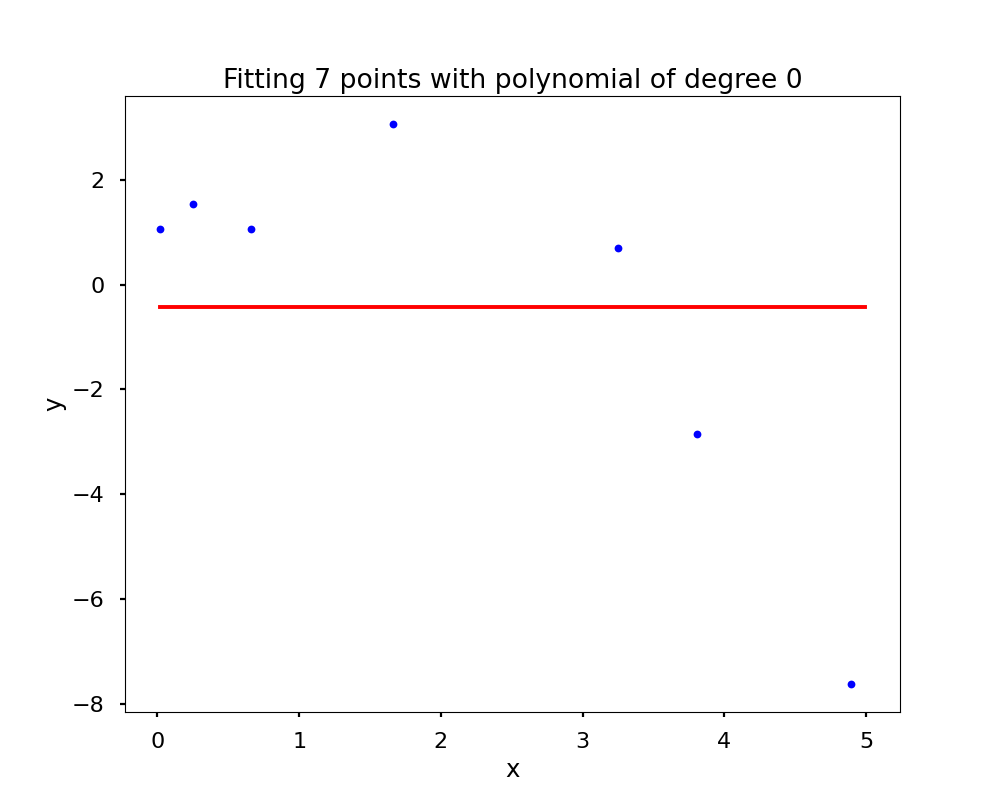
\includegraphics[width=5cm]{regression/1d-degree=0-train-fig.png}
        & 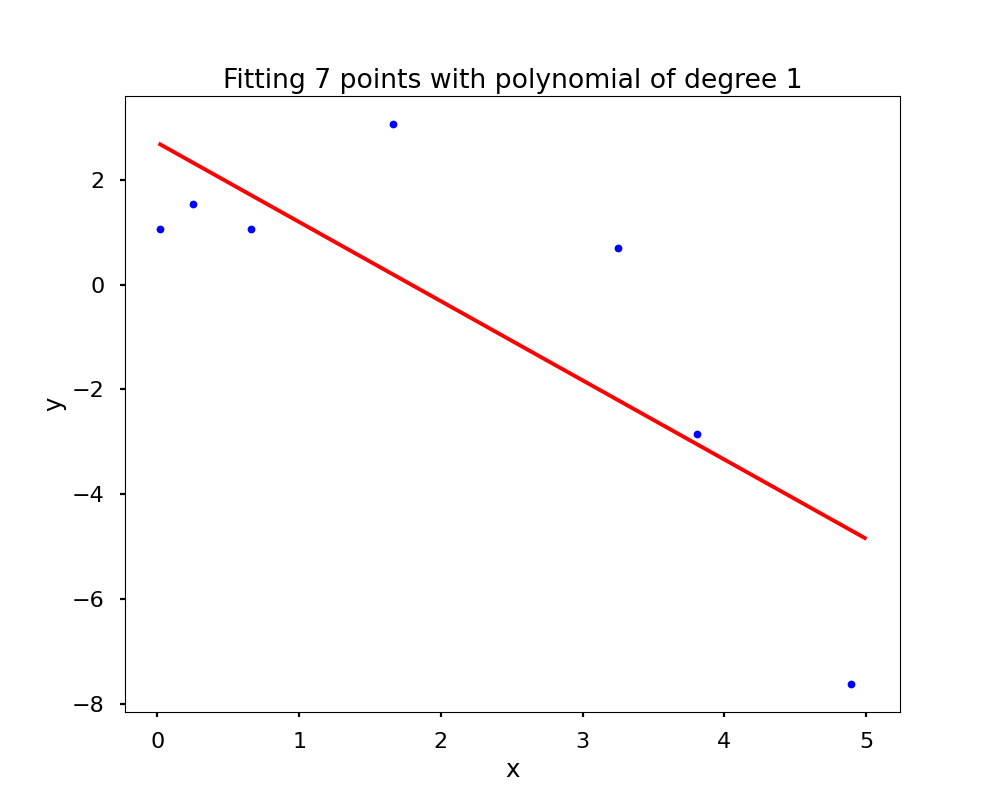
\includegraphics[width=5cm]{regression/1d-degree=1-train-fig.png}
        &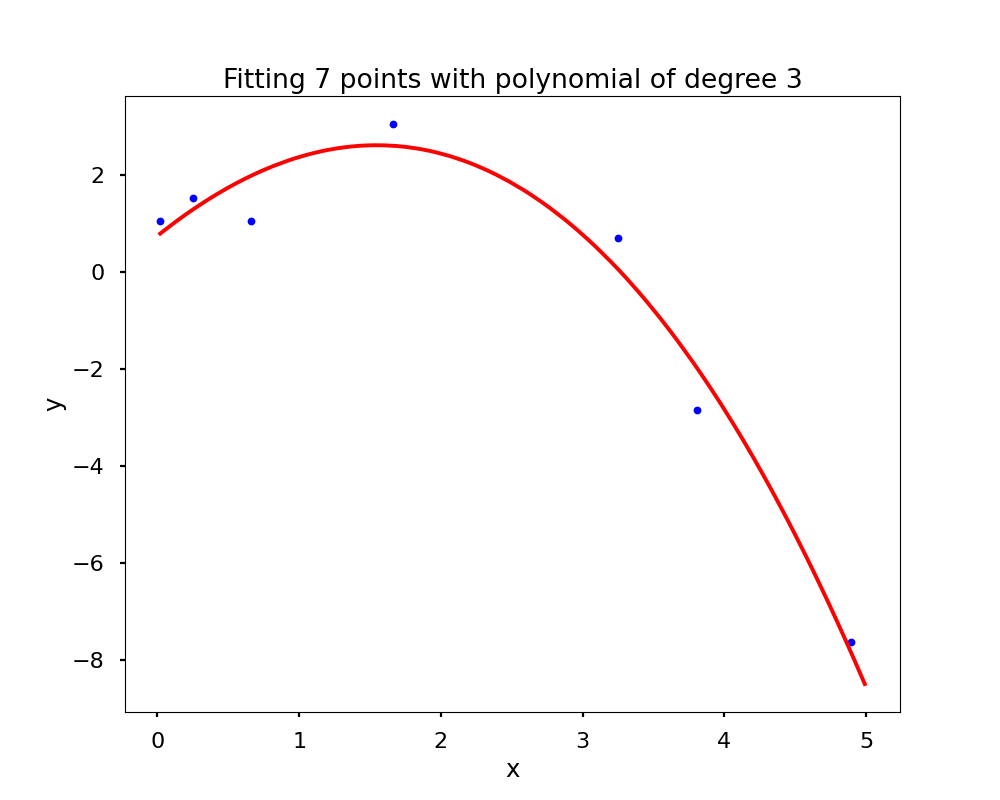
\includegraphics[width=5cm]{regression/1d-degree=3-train-fig.png}
          & 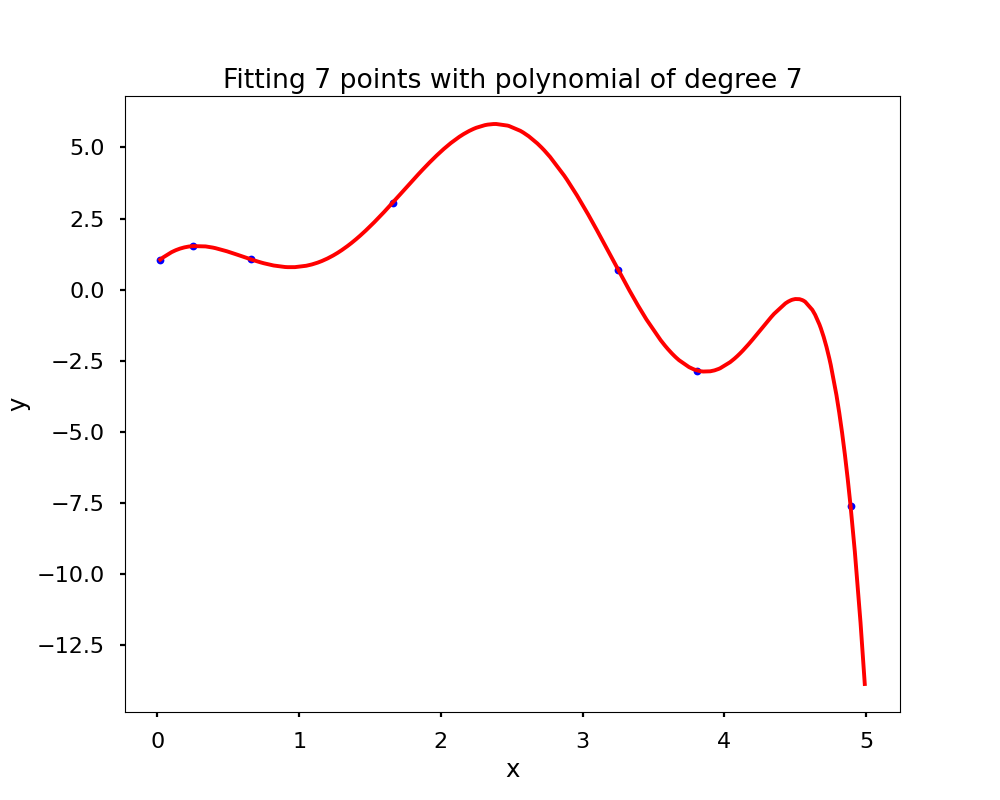
\includegraphics[width=5cm]{regression/1d-degree=7-train-fig.png}\\
          degree = 0 & degree = 1
          & degree = 3 & degree = 7\\
    \end{tabular}
\captionof{figure}{1D - Least Squares - Different degree polynomial fitted with 7 data points, cases of under-fitting and over-fitting.}
\end{center}

Figure 2 shows the results in case of 2D dataset.

% TODO: change this to add 2d images to it

\begin{center}
  \setlength\tabcolsep{0pt}
  \begin{tabular}{cccc}
    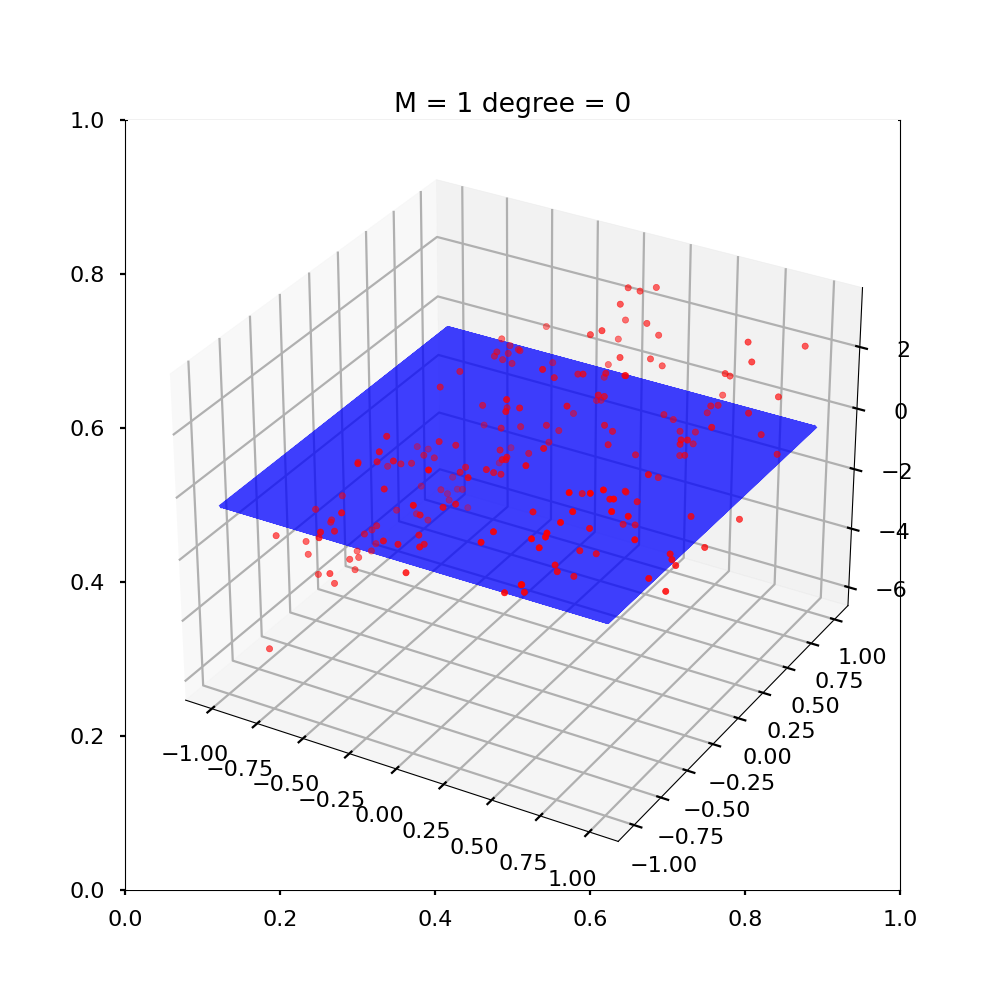
\includegraphics[width=5cm]{regression/2d-degree=0-train-fig.png}
      & 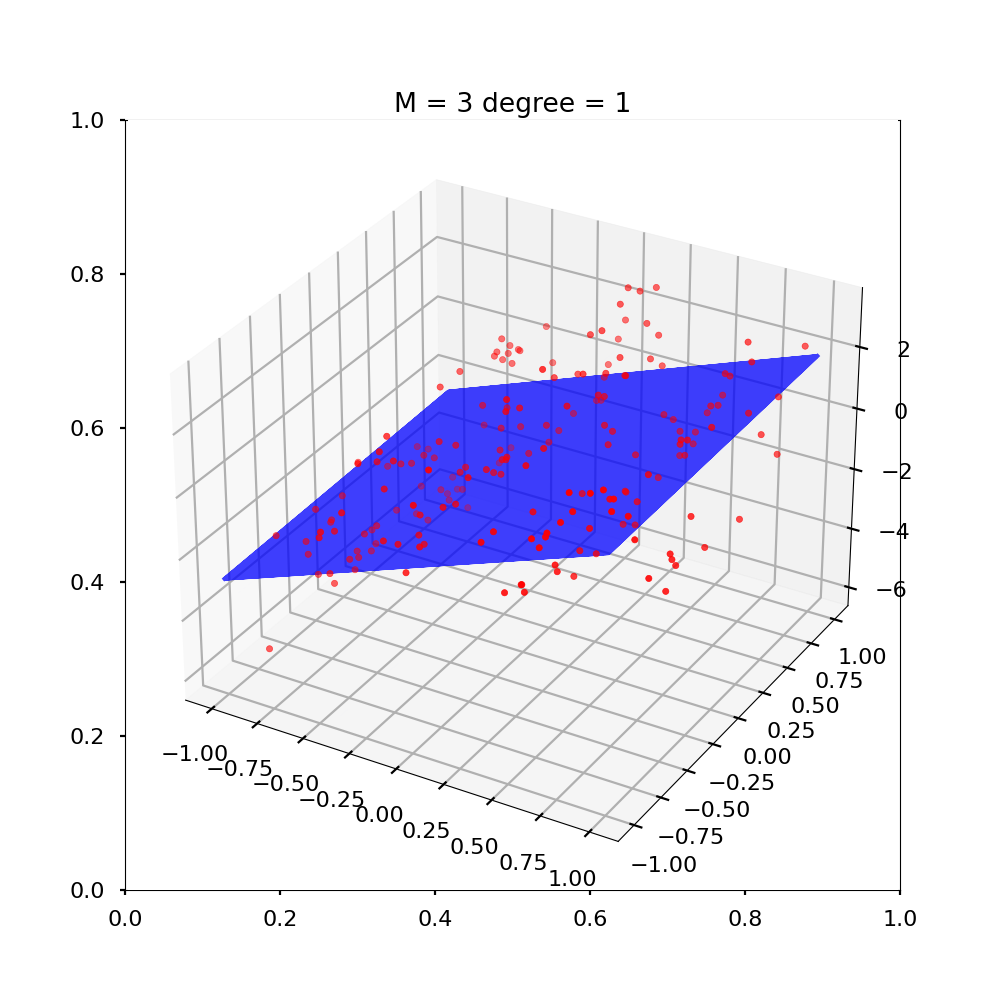
\includegraphics[width=5cm]{regression/2d-degree=1-train-fig.png}&
      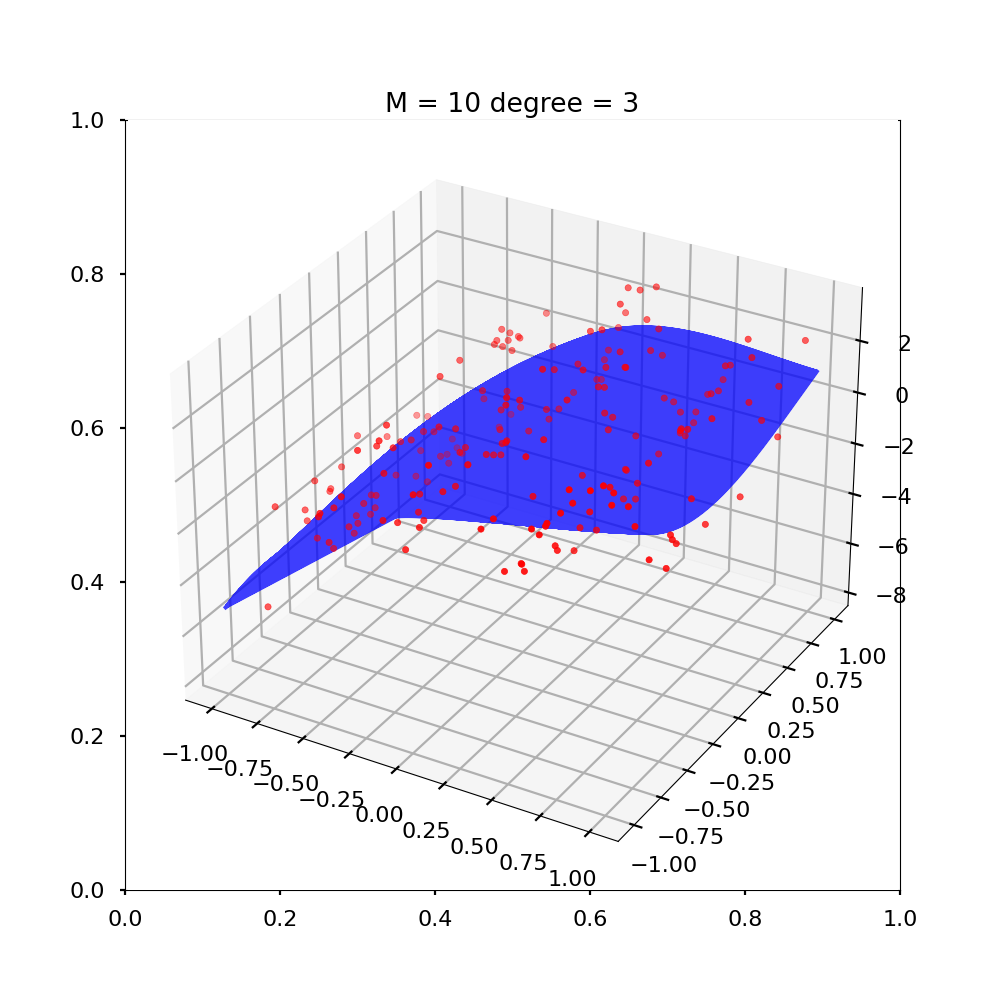
\includegraphics[width=5cm]{regression/2d-degree=3-train-fig.png}
        & 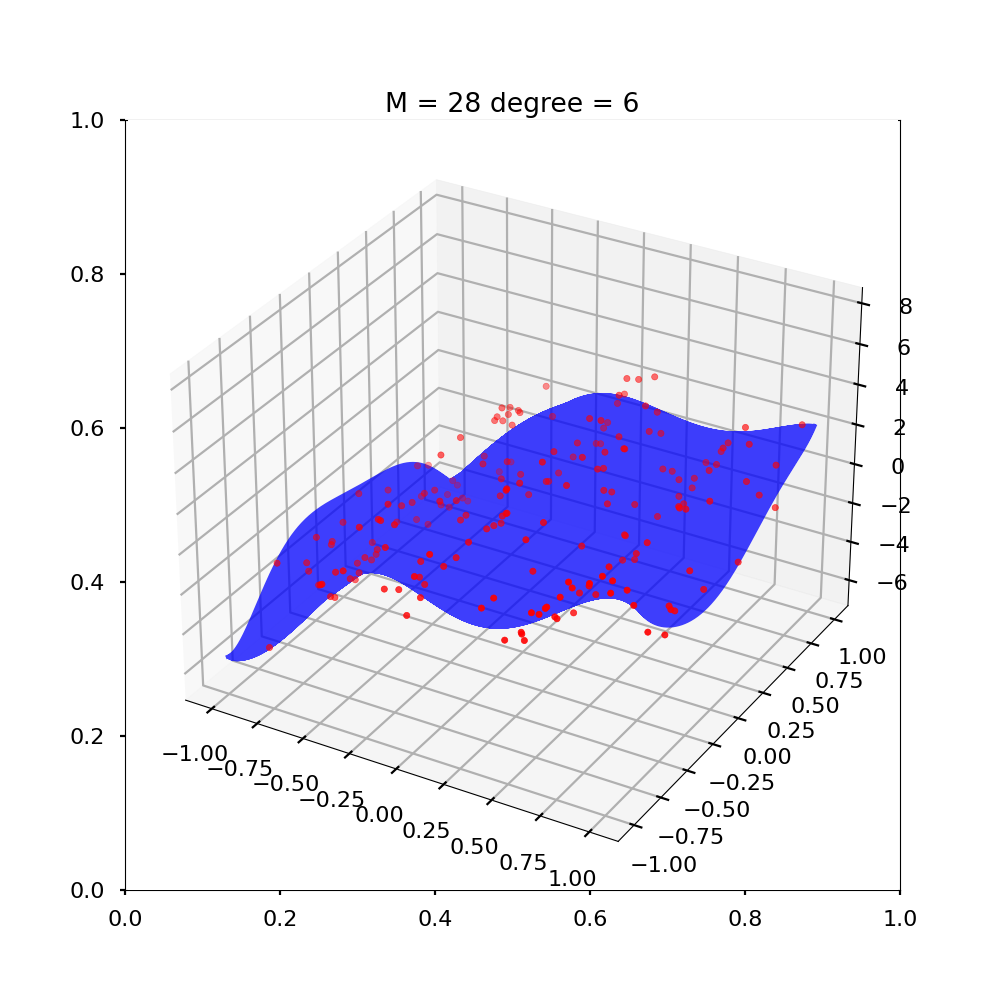
\includegraphics[width=5cm]{regression/2d-degree=6-train-fig.png}\\
      degree = 0 & degree = 1&
        degree = 3 & degree = 6\\
  \end{tabular}
\captionof{figure}{2D - Least Squares - Different degree polynomial fitted with 200 data points, cases of underfitting and overfitting.}
\end{center}

Figure 3 shows the RMS Error trend in the training and development sets, as the parameter M varies. This is for 1D dataset.

\begin{center}
  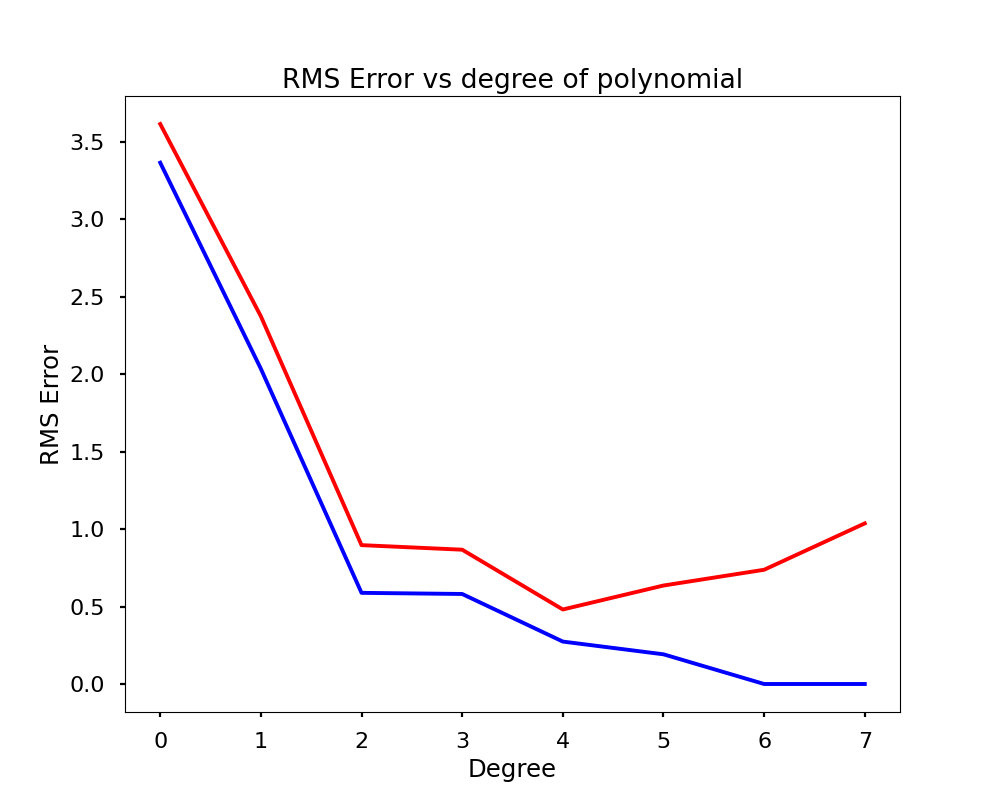
\includegraphics[width=10cm]
  {regression/1d-ls-train-dev-fig.png}
  \captionof{figure}{RMS Error vs degree plots for training (blue) and development (red) data (1D dataset)}   
\end{center}

Figure 4 shows the RMS Error trend in the training and development sets, as the parameter M varies. This is for 2D dataset.

\begin{center}
  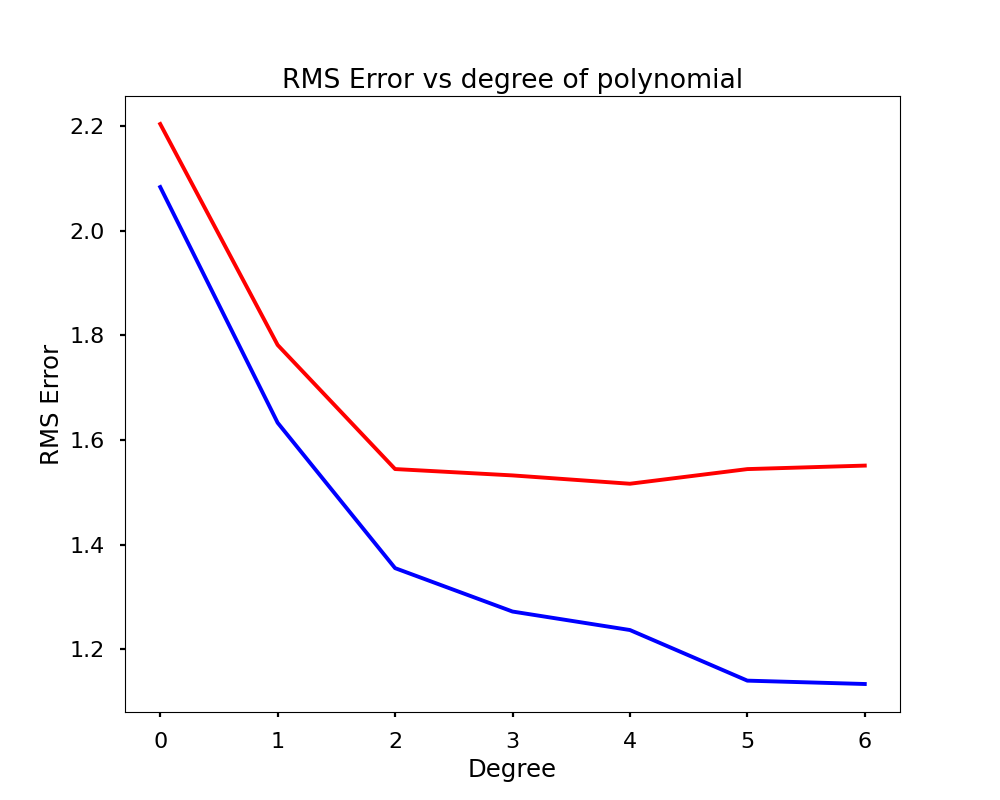
\includegraphics[width=10cm]
{regression/2d-ls-train-dev-fig.png}
\captionof{figure}{RMS Error vs degree plots for training (blue) and development (red) data (2D dataset)}
\end{center}


\section*{Experiment 2}
We now expand the training set, i.e, vary the number of training samples, and we choose the M with the lowest RMS Error. Figure 5 shows the results for 1D dataset.

\begin{center}
\setlength\tabcolsep{0pt}
\begin{tabular}{cccc}
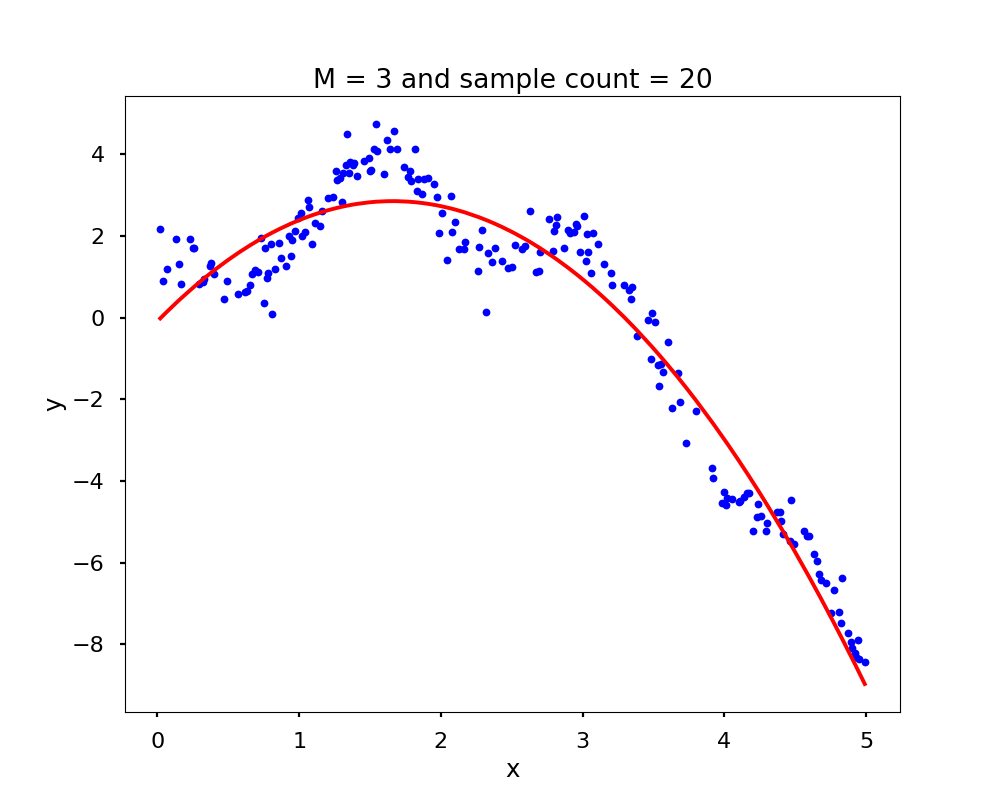
\includegraphics[width=5cm]{regression/1d-complex-20-dev-fig.png}
& 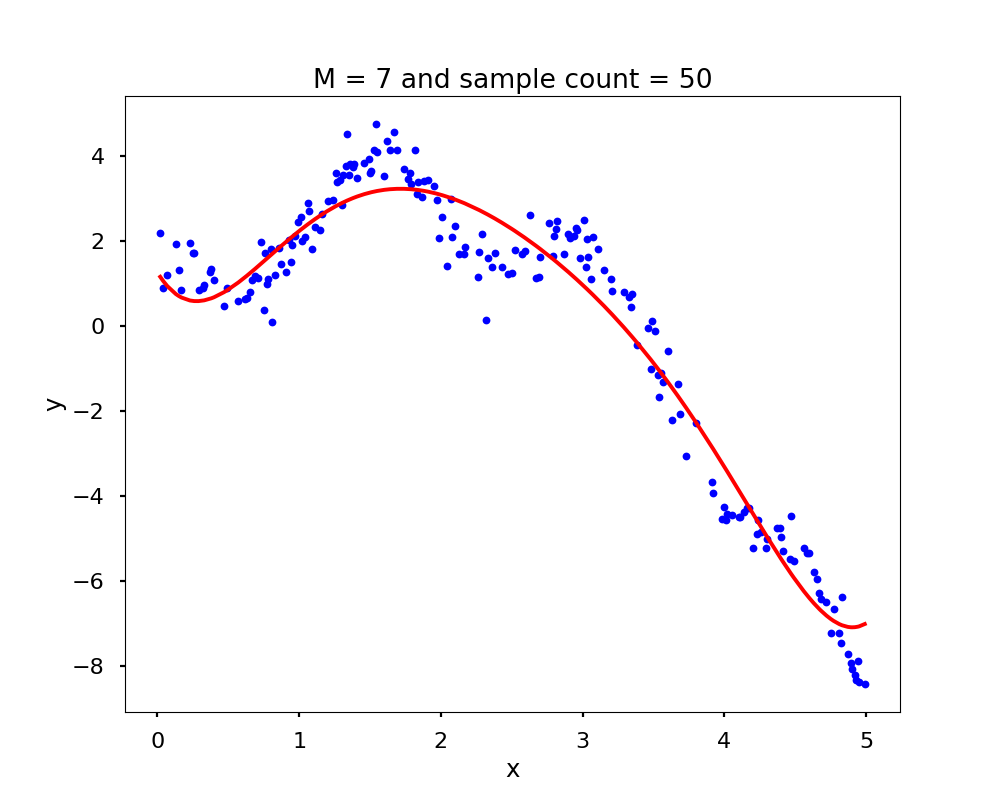
\includegraphics[width=5cm]{regression/1d-complex-50-dev-fig.png}
& 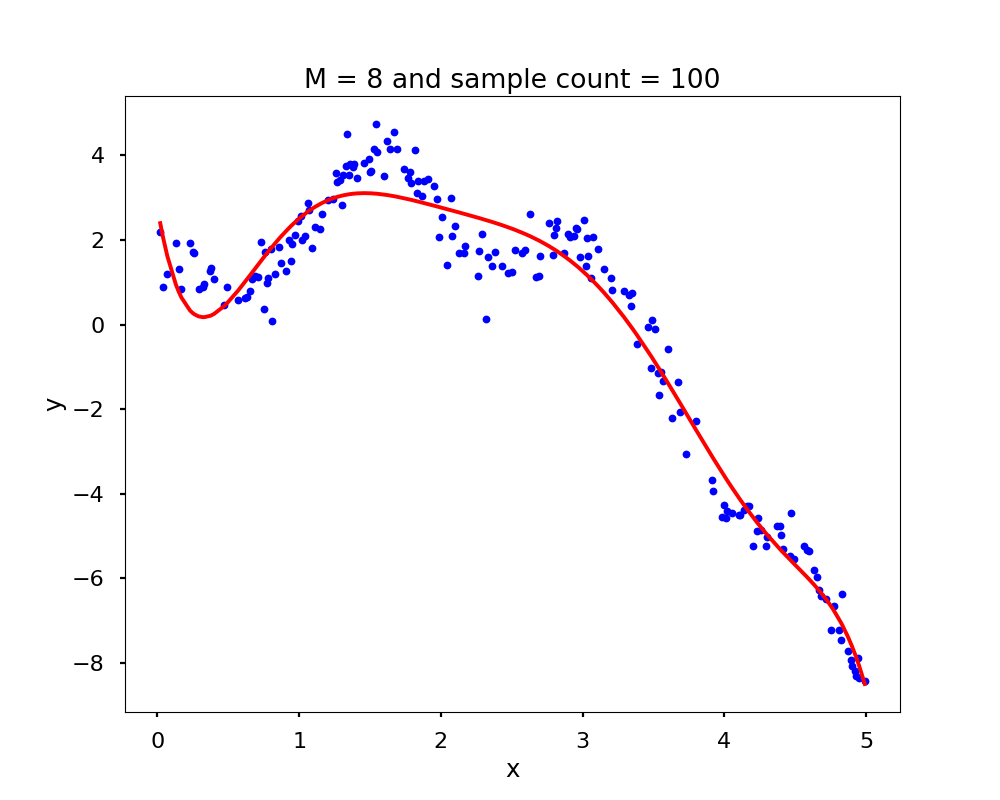
\includegraphics[width=5cm]{regression/1d-complex-100-dev-fig.png}
& 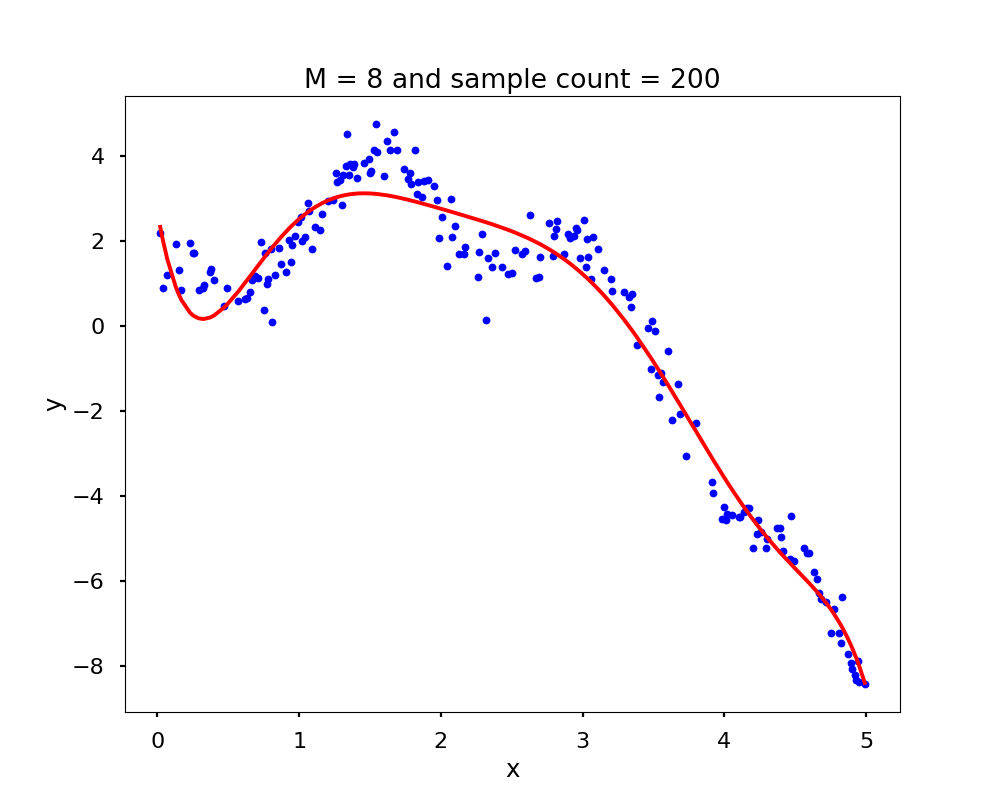
\includegraphics[width=5cm]{regression/1d-complex-200-dev-fig.png}\\
sample size = 20 & sample size = 50
& sample size = 100 & sample size = 200 \\
\end{tabular}
\captionof{figure}{1D - Least Squares - Different sample sizes of training data}
\end{center}

Figure 6 shows the results for the same experiment with 2D dataset.

% TODO: put images of 2d dataset
\begin{center}
  \setlength\tabcolsep{0pt}
  \begin{tabular}{cccc}
  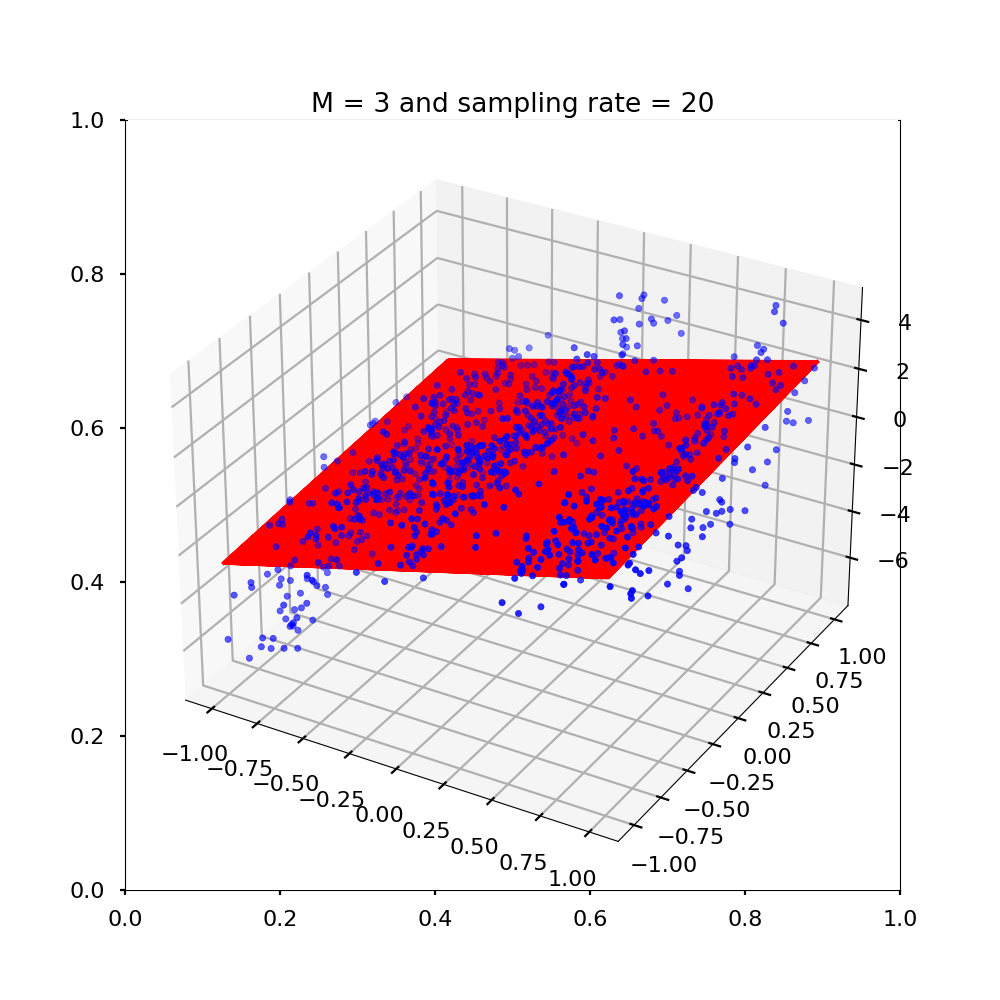
\includegraphics[width=5cm]{regression/2d-ls-20-test-fig.png}
  & 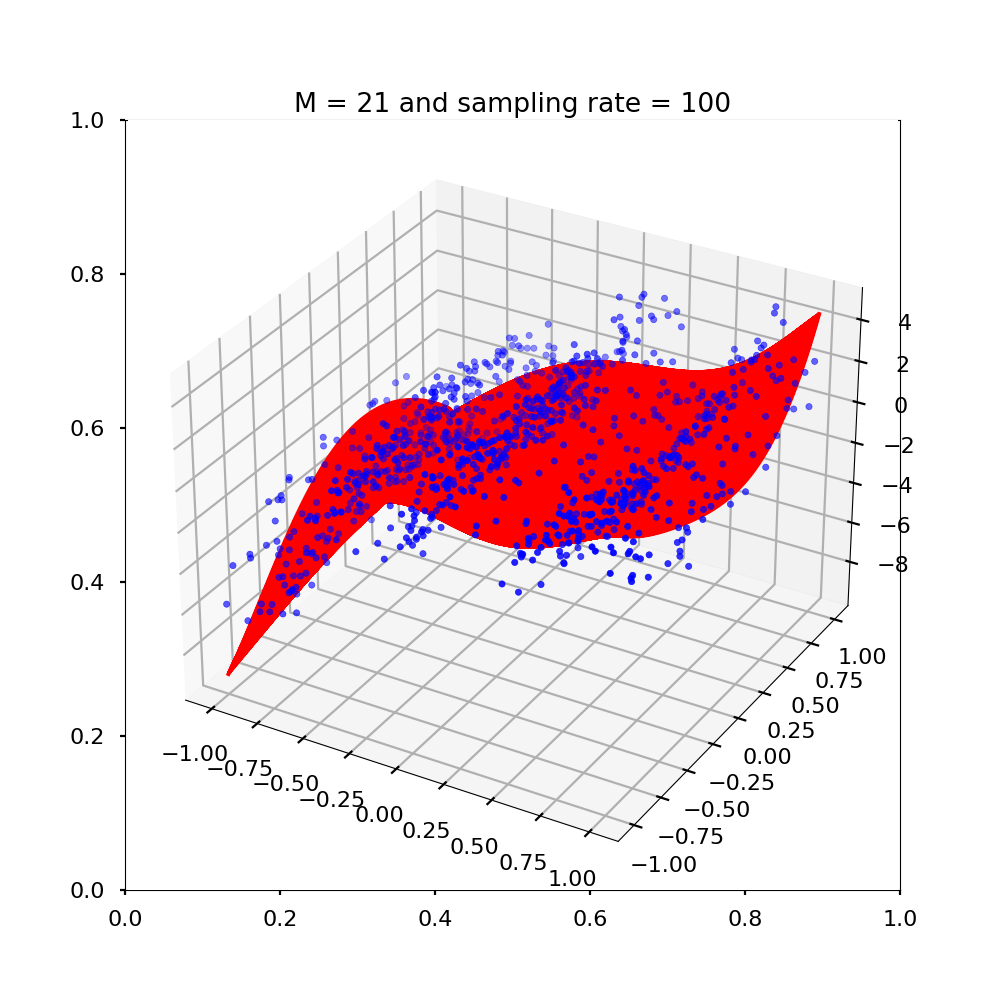
\includegraphics[width=5cm]{regression/2d-ls-100-test-fig.png}&
  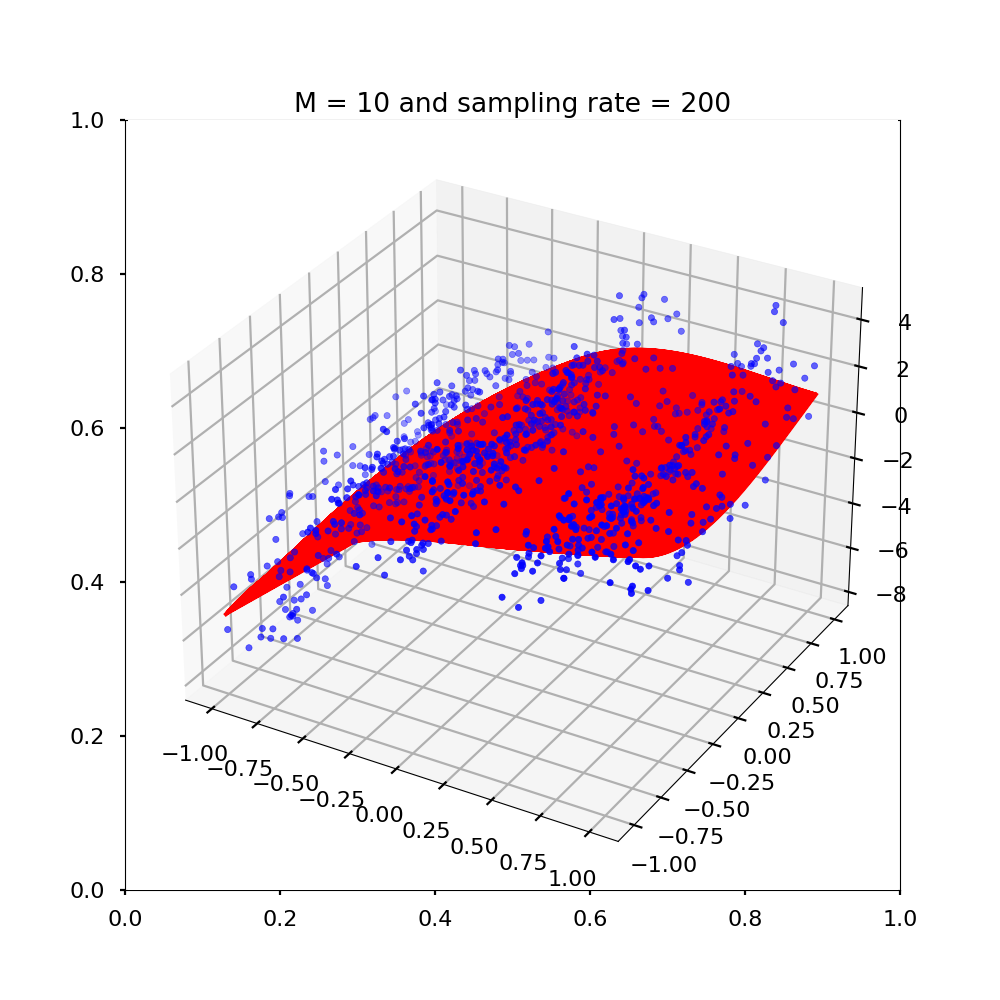
\includegraphics[width=5cm]{regression/2d-ls-200-test-fig.png}
  & 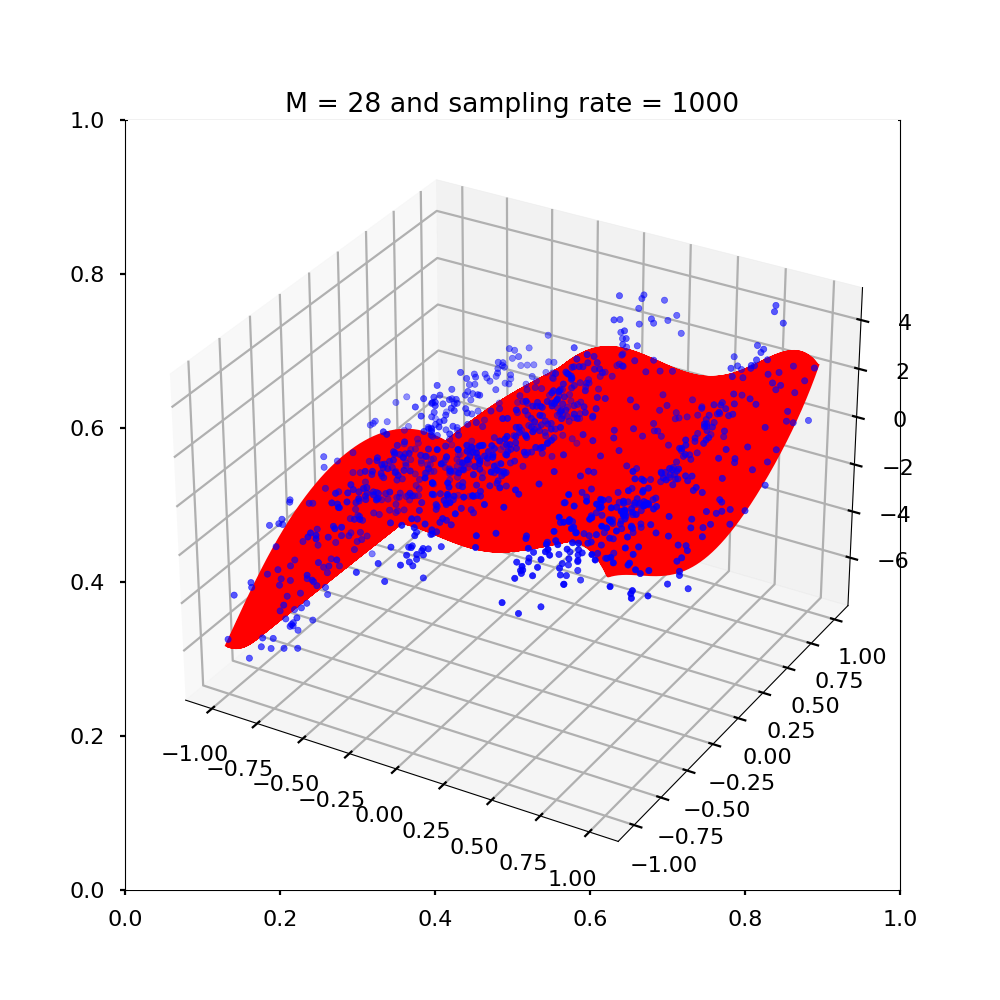
\includegraphics[width=5cm]{regression/2d-ls-1000-test-fig.png}\\
  sample size = 20 & sample size = 100&
  sample size = 200 & sample size = 1000 \\
  \end{tabular}
  \captionof{figure}{1D - Least Squares - Different sample sizes of training data}
  \end{center}

Figure 7 shows the RMS value affected on the development set by the varying sample size.

\begin{center}
  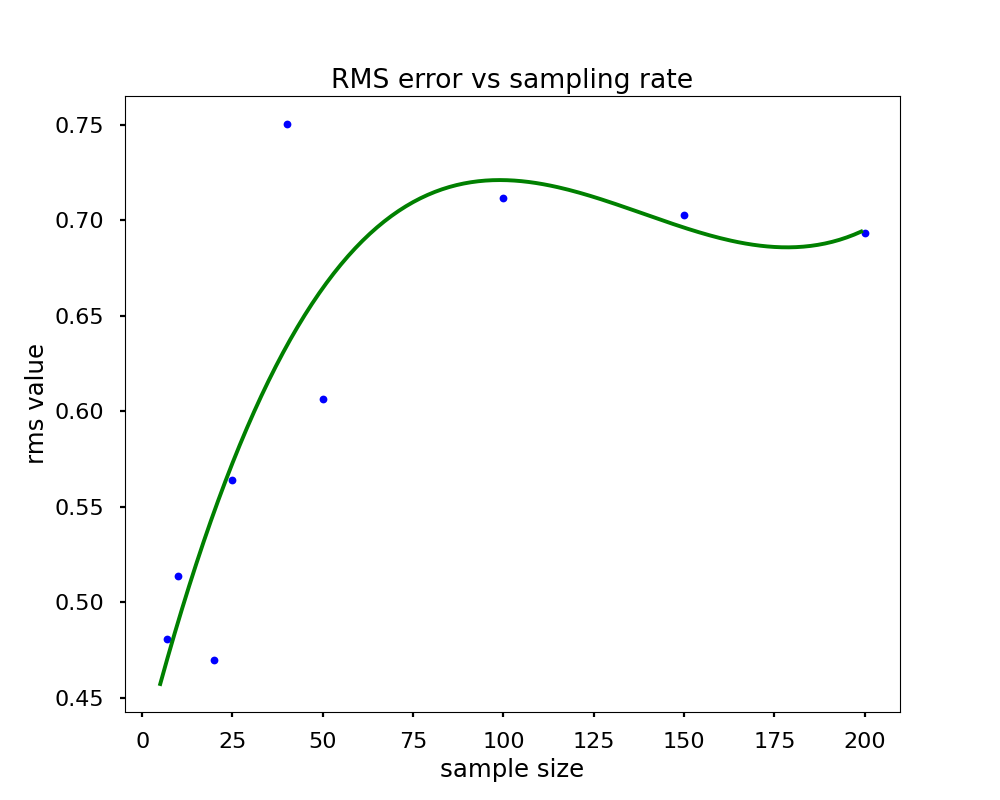
\includegraphics[width=8cm]
{regression/1d-rms-vs-sample-size-fig.png}
\captionof{figure}{RMS Error vs sample size for 1D dataset}
\end{center}

This plot is not the kind we expected for real data. This is because this is not real data, and the noise is not completely random in this dataset.
To produce good results in this case, we divided the dataset into several batches of mentioned sizes, and took the average of corresponding coefficients over all the batches.
As a result, even smaller sample sizes are performing better, even better than large ones.

Figure 8 shows the same plot for 2D dataset.

\begin{center}
  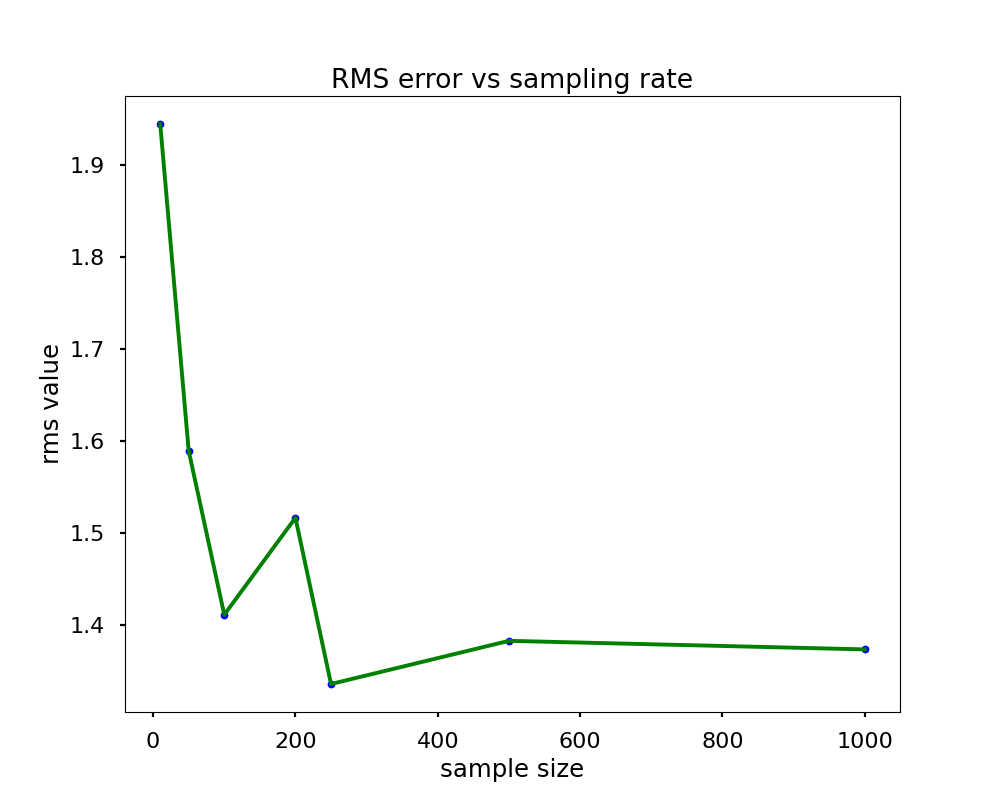
\includegraphics[width=8cm]
{regression/2d-rms-vs-sample-size-fig.png}
\captionof{figure}{RMS Error vs sample size for 2D dataset}
\end{center}

It can be seen that the above 2D dataset diagram represents expected behaviour more closely than the one for 1D dataset. This, however, is purely due to the nature of the data, and we don't expect this in general.

\section*{Experiment 3}

We introduced regularization with quadratic error (ridge regression). Using several values of regularization parameter \(\lambda\), we observed the changes it made in the fit polynomial of different degrees. As results, we present here with 4 values of \(\lambda\) used on different degrees of polynomial.

Figure 9 shows 1D dataset polynomial fit with 7 points and degree 6.

\begin{center}
  \setlength\tabcolsep{0pt}
  \begin{tabular}{ccc}
  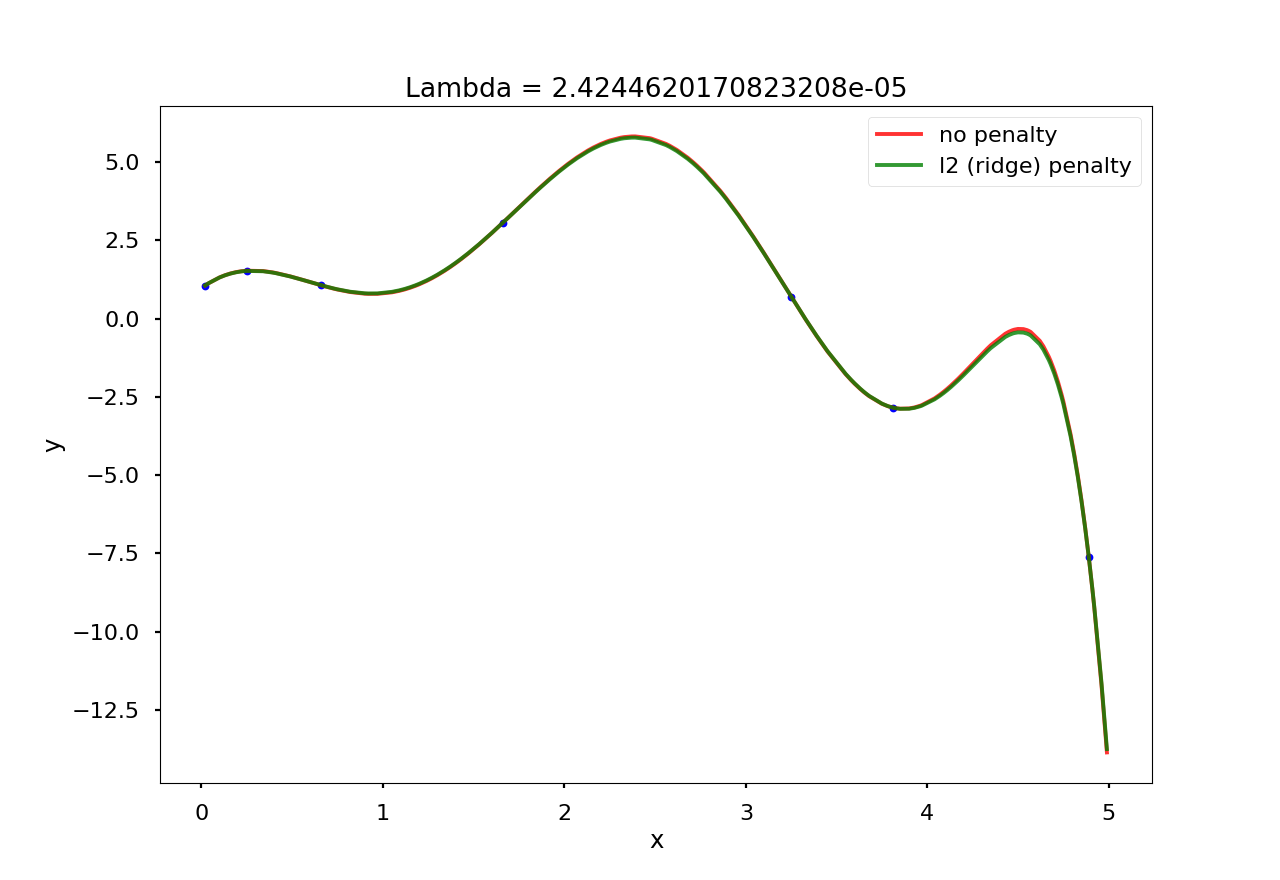
\includegraphics[width=7cm]{regression/1d-ridge-ls-compare-7-7lnlam--4.615384615384617-fig.png}
  & 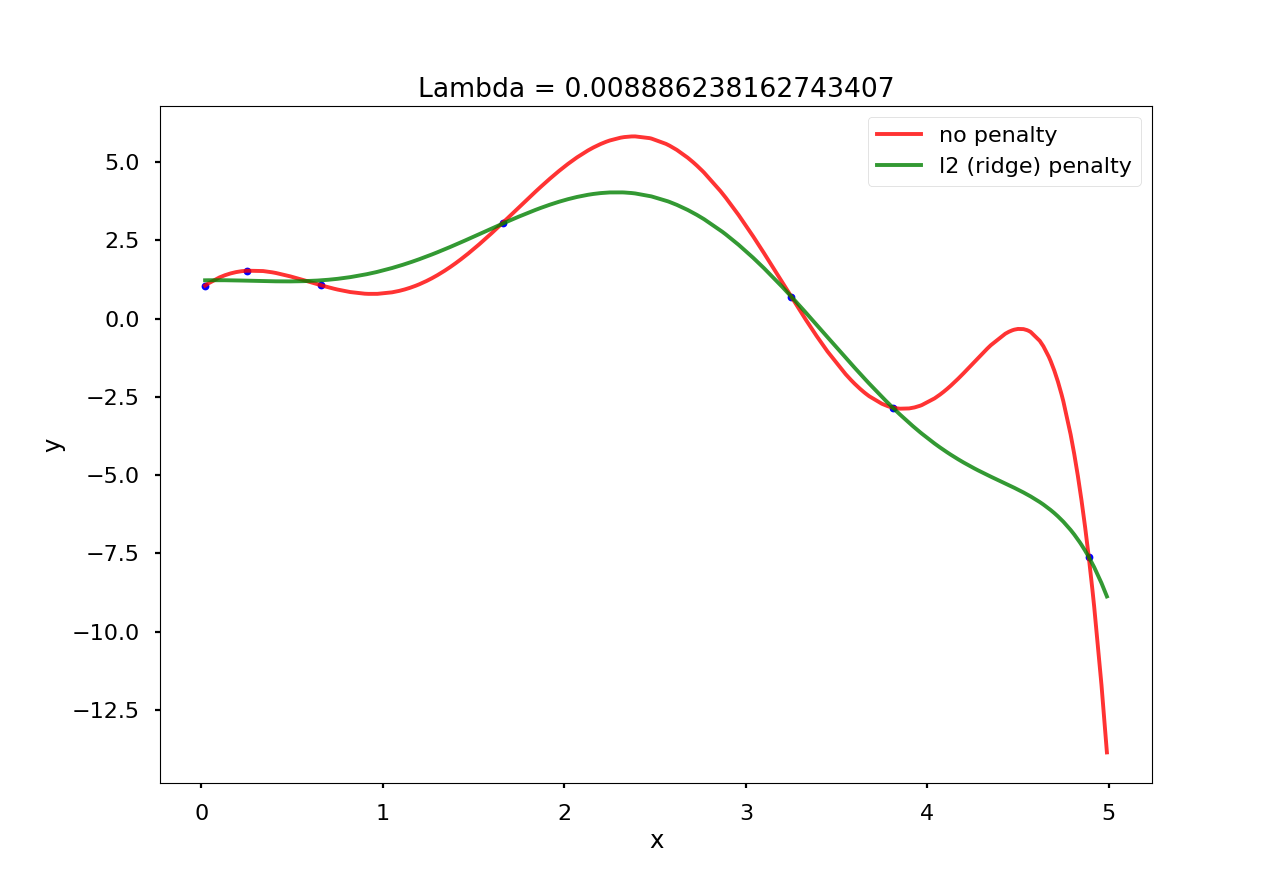
\includegraphics[width=7cm]{regression/1d-ridge-ls-compare-7-7lnlam--2.051282051282051-fig.png}\\
  sample size = 20 & sample size = 100\\
  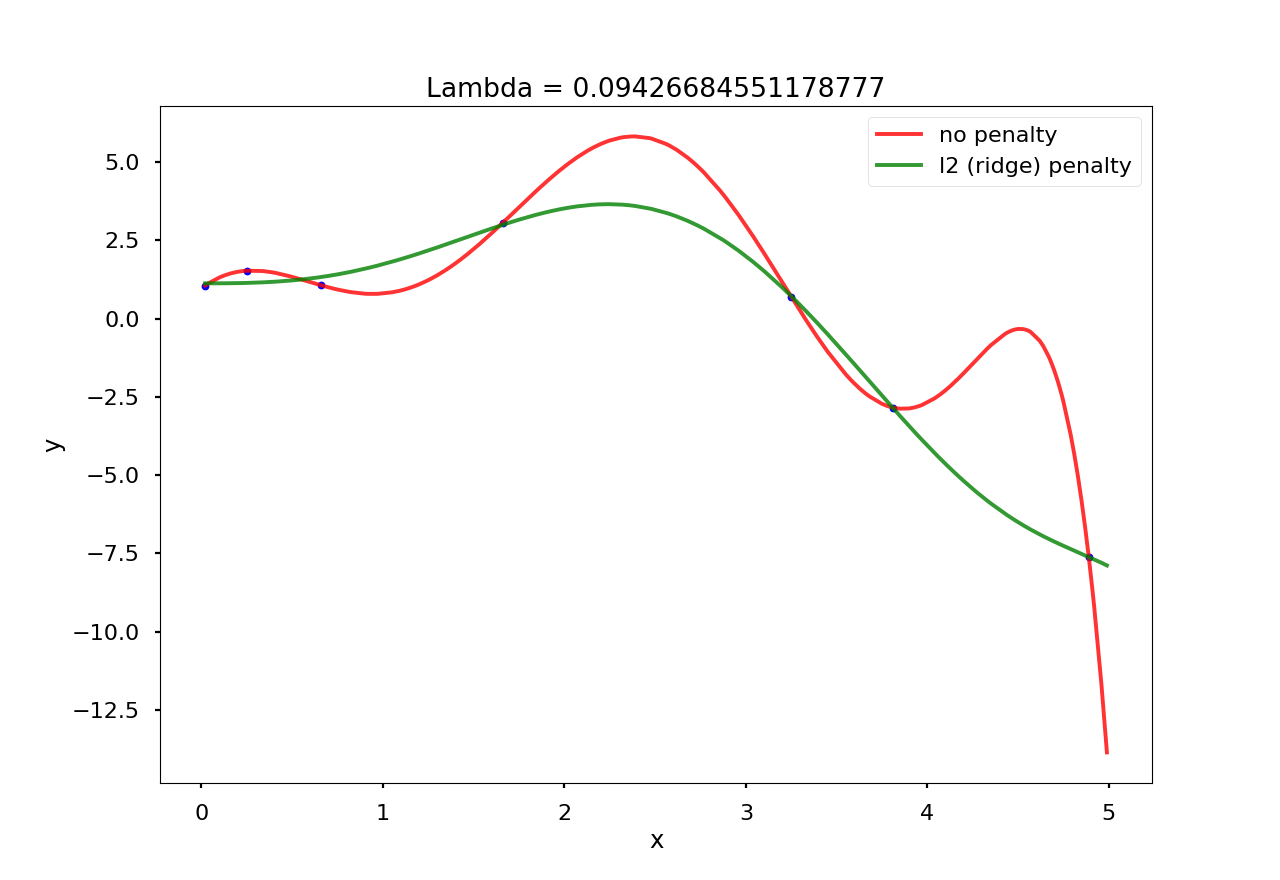
\includegraphics[width=7cm]{regression/1d-ridge-ls-compare-7-7lnlam--1.025641025641029-fig.png}
  & 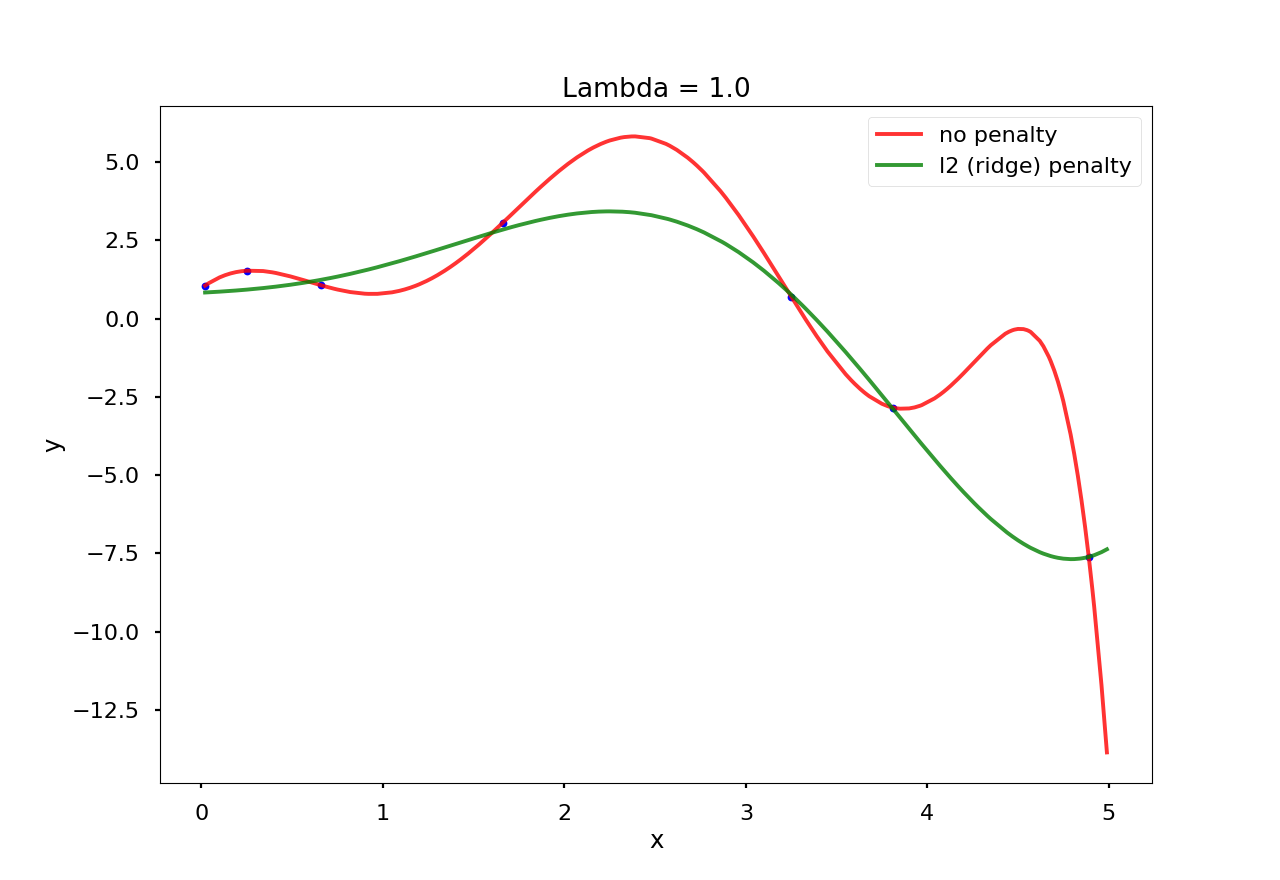
\includegraphics[width=7cm]{regression/1d-ridge-ls-compare-7-7lnlam-0.0-fig.png}\\
  sample size = 200 & sample size = 1000 \\
  \end{tabular}
  \captionof{figure}{1D - Difference in the least squares approach and ridge regression.}
\end{center}
  Similarly, we computed the regression fit for 2D dataset. Figure 10 shows polynomial fit on 2D dataset with 200 points and degree 6.

  \begin{center}
    \setlength\tabcolsep{0pt}
    \begin{tabular}{ccc}
    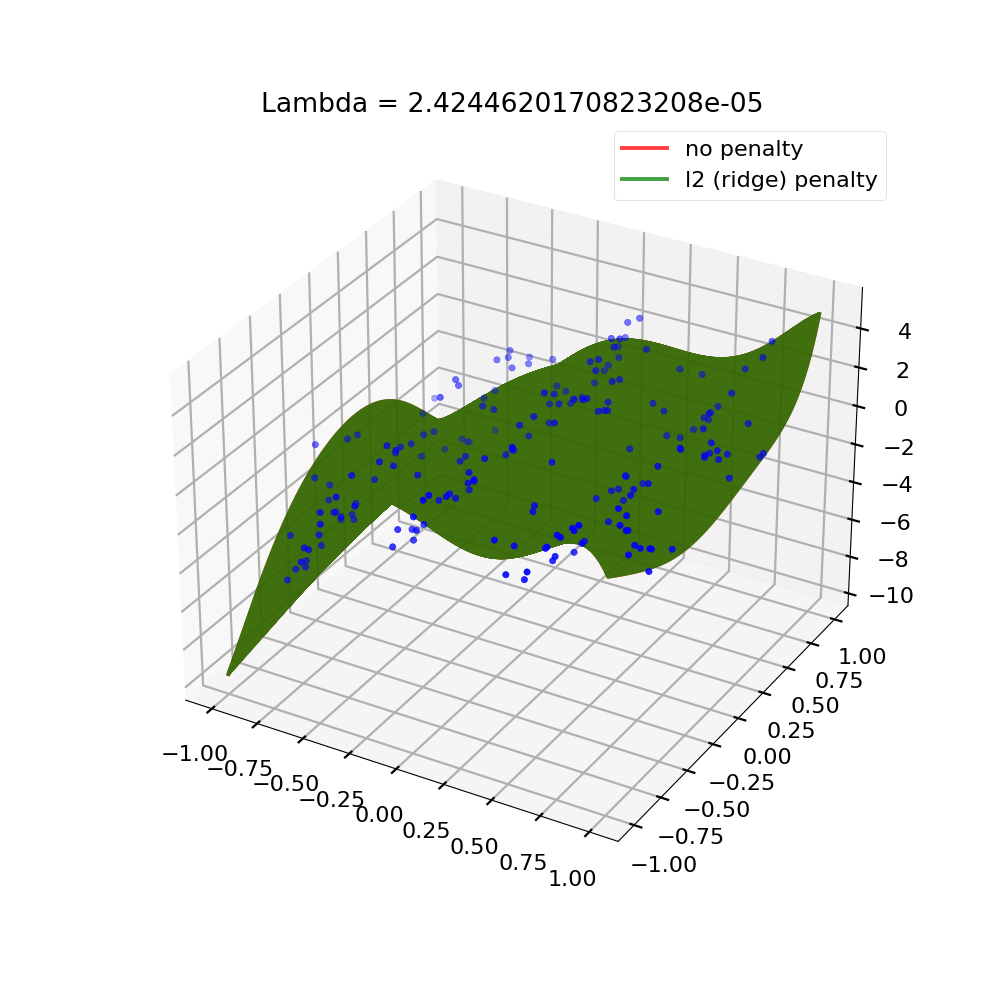
\includegraphics[width=7cm]{regression/2d-ridge-ls-compare-27-200lnlam--4.615384615384617-fig.png}
    & 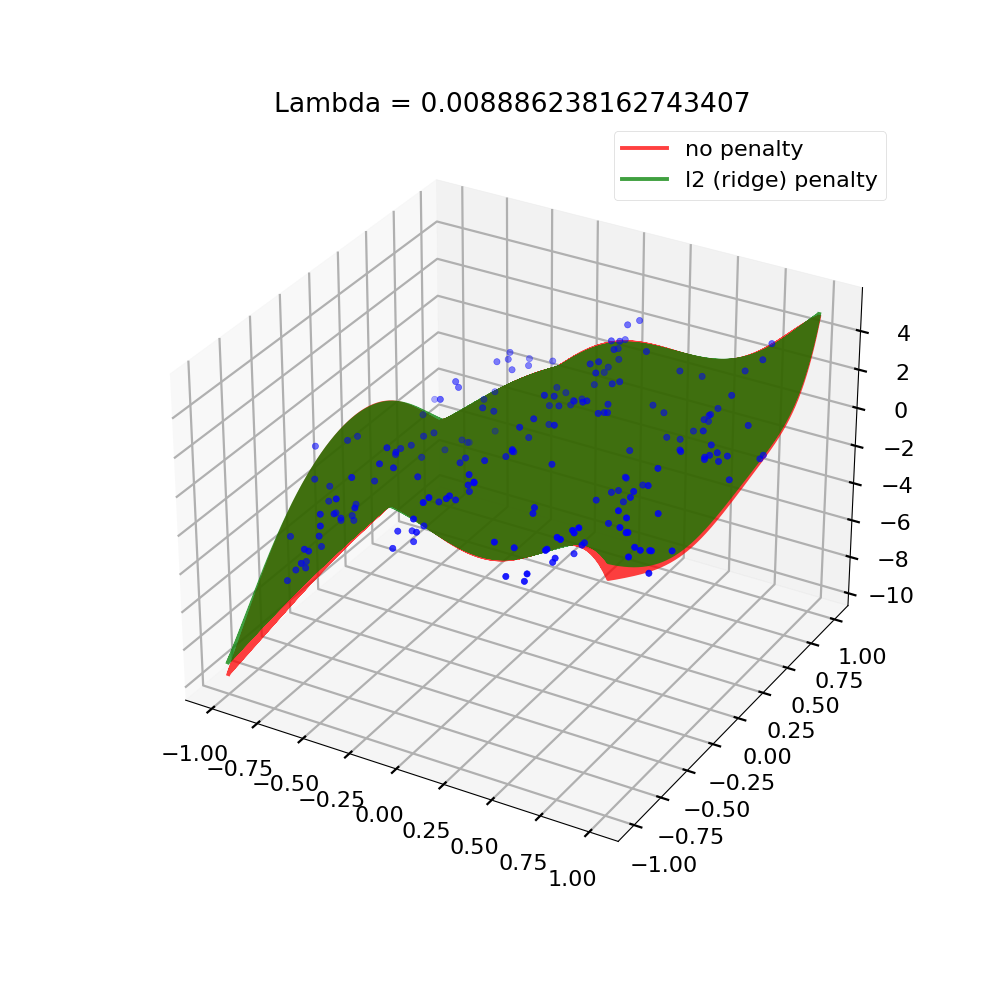
\includegraphics[width=7cm]{regression/2d-ridge-ls-compare-27-200lnlam--2.051282051282051-fig.png}\\
    sample size = 20 & sample size = 100\\
    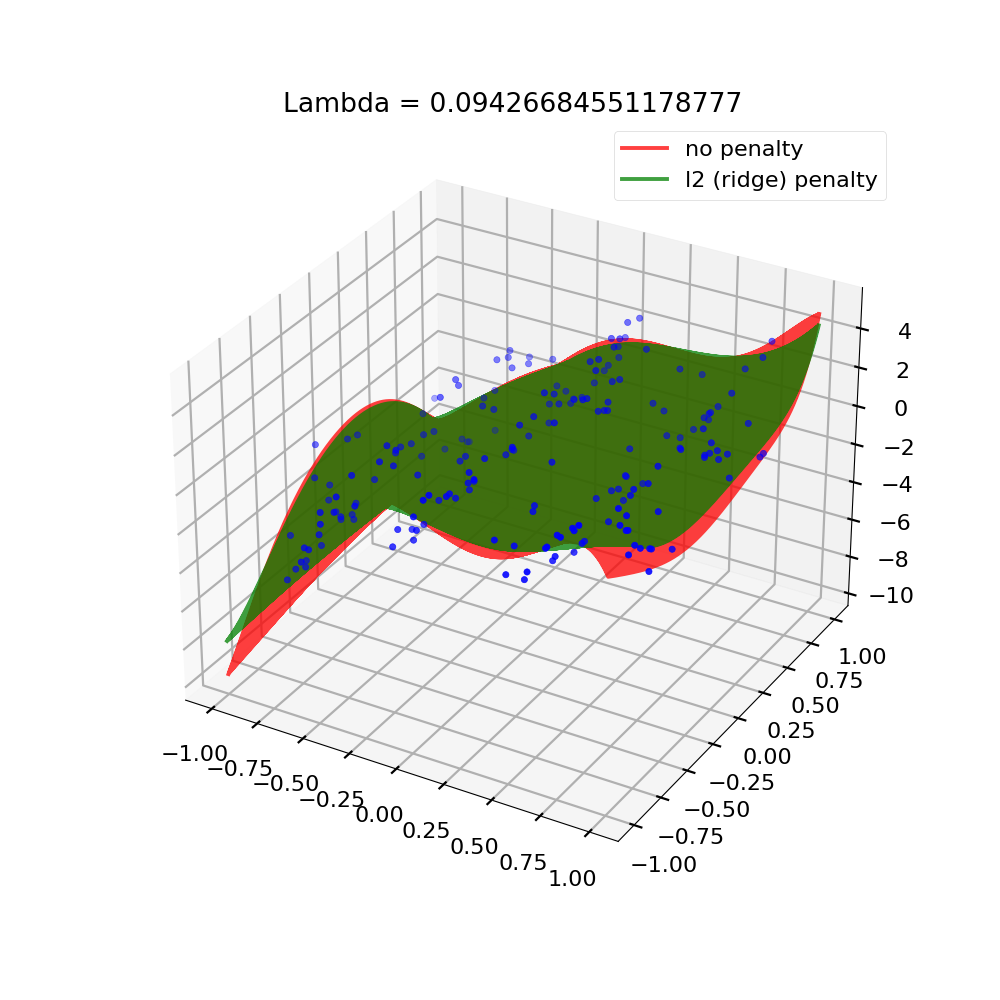
\includegraphics[width=7cm]{regression/2d-ridge-ls-compare-27-200lnlam--1.025641025641029-fig.png}
    & 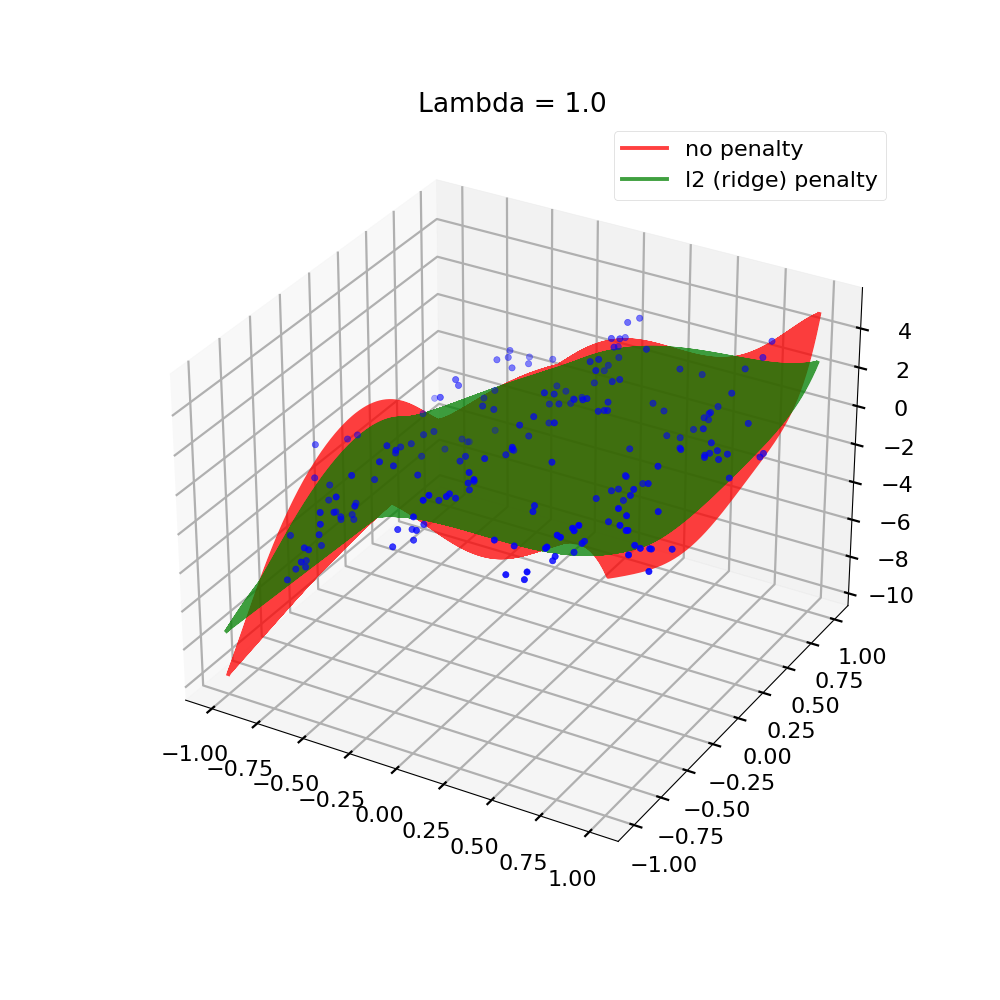
\includegraphics[width=7cm]{regression/2d-ridge-ls-compare-27-200lnlam-0.0-fig.png}\\
    sample size = 200 & sample size = 1000 \\
    \end{tabular}
    \captionof{figure}{2D - Difference in the least squares approach and ridge regression.}
  \end{center}
From above figures, it is clearly evident how ridge regression uses l2 penalty to avoid the over-fitting that we observed in plain least square regresssion. 

Figure 11 shows how RMS error reduces the error on development data for different values of lambda on 1D data. It reached its lowest when log lambda was somewhere between -2.5 and 0.0.

\begin{center}
  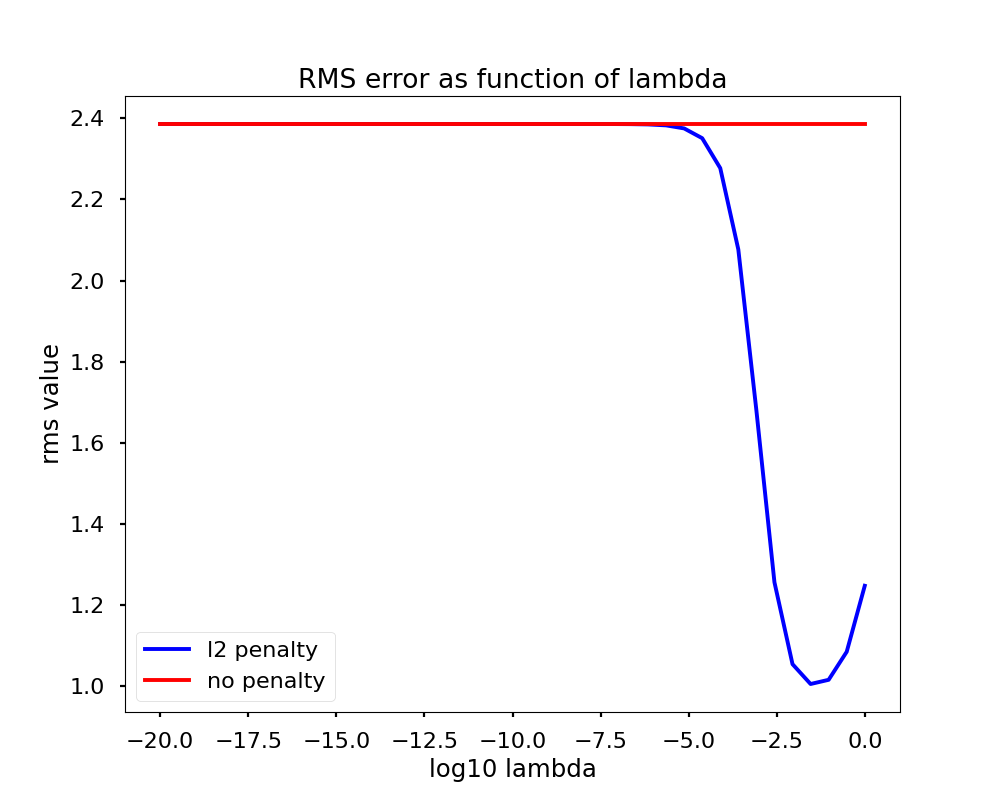
\includegraphics[width=10cm]
  {regression/1d-rms-vs-lam-fig.png}
  \captionof{figure}{RMS Error vs log lambda for 1D dataset}
\end{center}

Figure 12 shows the same statistic for 2D dataset.

\begin{center}
  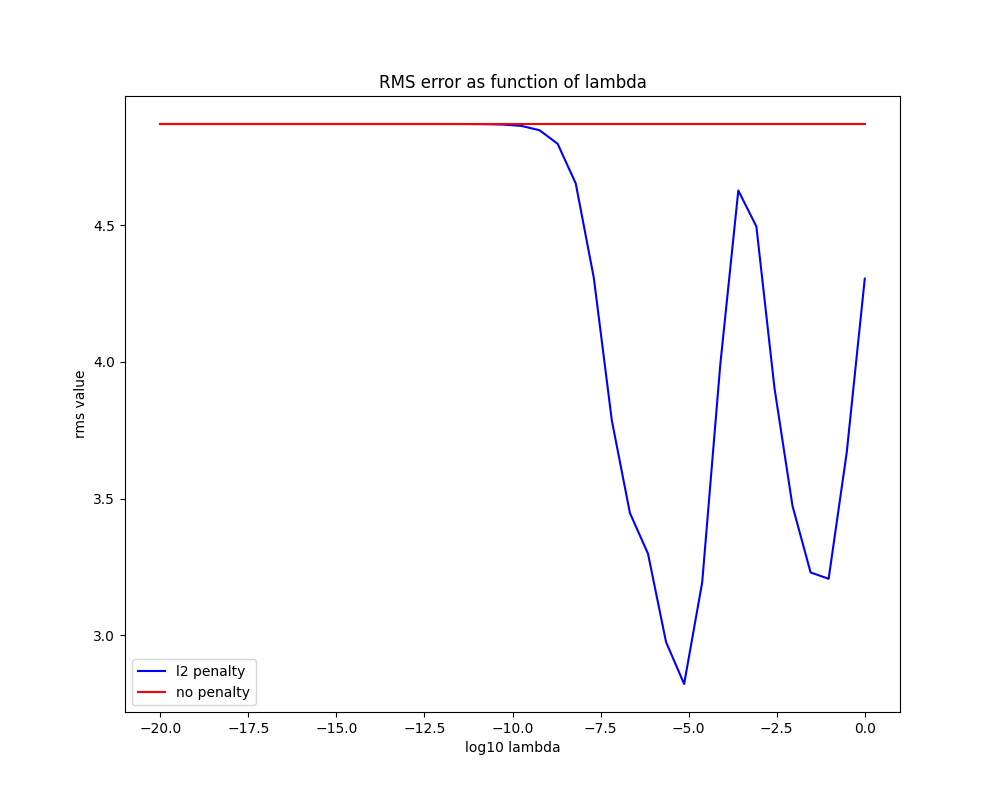
\includegraphics[width=10cm]
  {regression/2d-rms-vs-lam-fig.png}
  \captionof{figure}{RMS Error vs log lambda for 2D dataset}
\end{center}

In this paper we looked at linear regression, and the various results obtained by changing
\begin{packed_enum}
  \item the hyperparameter M, which is the dimension of the weight vector
  \item the hyperparameter \(\lambda\), which is the regularization constant
  \item the sample sizes for training the model
\end{packed_enum}

We also noted that the noise in the data wasn't completely random, in which case, we decided to split the training data randomly into several smaller samples, and then find the polynomial fit for each of them, and finally average the corresponding coefficients of the weight vector.

After that, we fine-tuned the hyperparameters by evaluating it on development data. Note that in all observations in this paper, the seed of the randomizer was fixed (value 6), to maintain consistency of the results. In practise, we prefer to not specify the seed.

\newpage
\begin{center}
\title*{\LARGE \textbf{(B) Bayesian Classifier}}
\end{center}
We use the abbreviations - LS for Linearly Separable Data, NLS - Non Linearly Separable Data, and RE for Real Data. We also use the Ci, as a data type suffix, for indicating that the plot belongs is for Case i as in the assignment statement. So, NLSC1 indicates Case 1 of NLS data. The most exciting plots were generated by Real Data and hence, we will focus on it. From training data, we see that the prior is an uniform distribution on the classes.
\section*{Probability Density Functions:-}
We will first look at some sample PDFs from what we plotted for the 5 cases and 3 types of data.
\begin{center}
  \setlength\tabcolsep{-7pt}
  \begin{tabular}{cccc}
  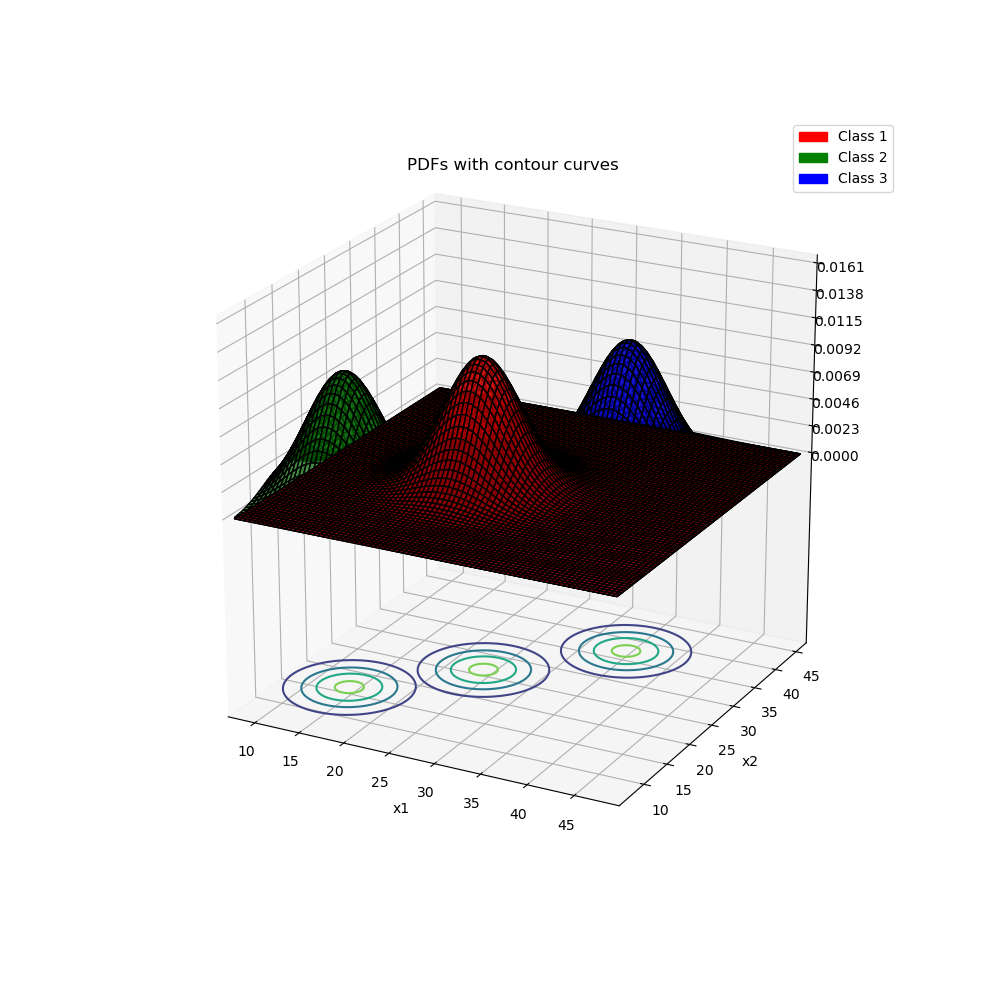
\includegraphics[width=5.5cm]{classifier/PDFs/NLS/case3.png}
  & 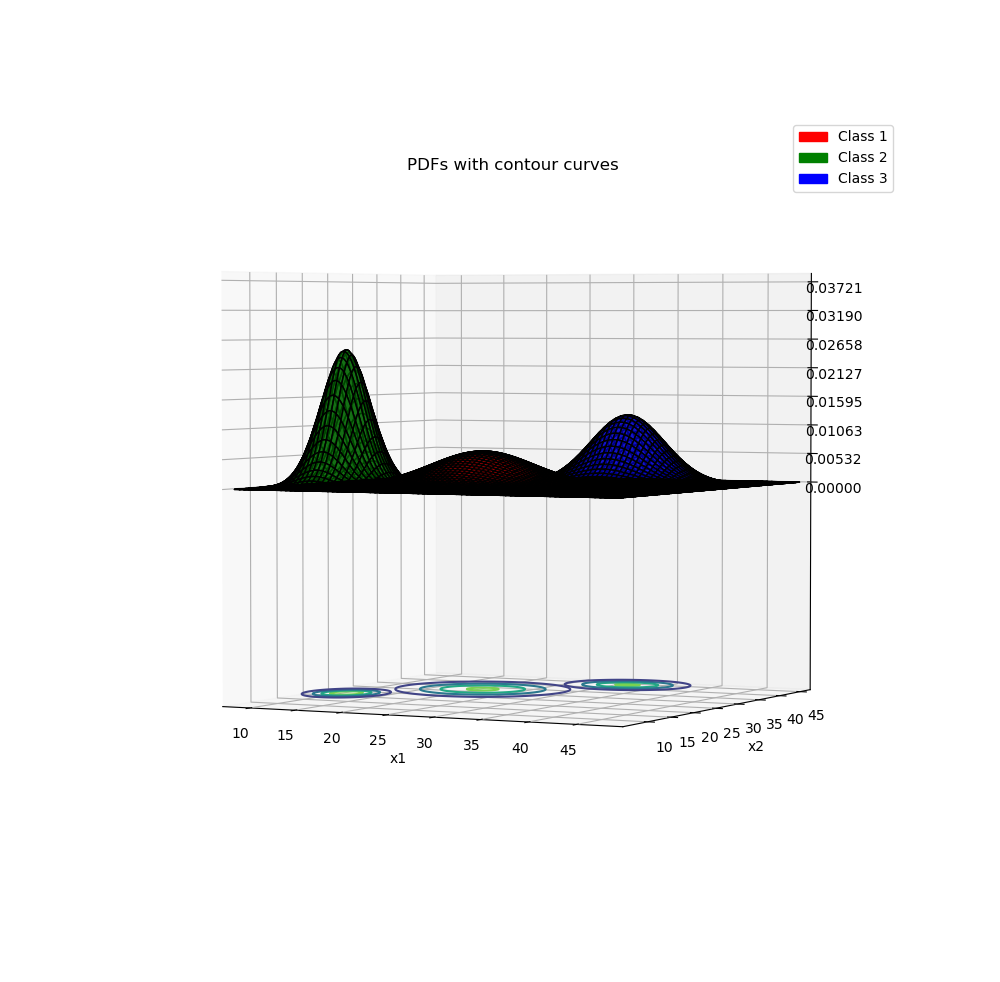
\includegraphics[width=5.5cm]{classifier/PDFs/NLS/case5.png}
  & 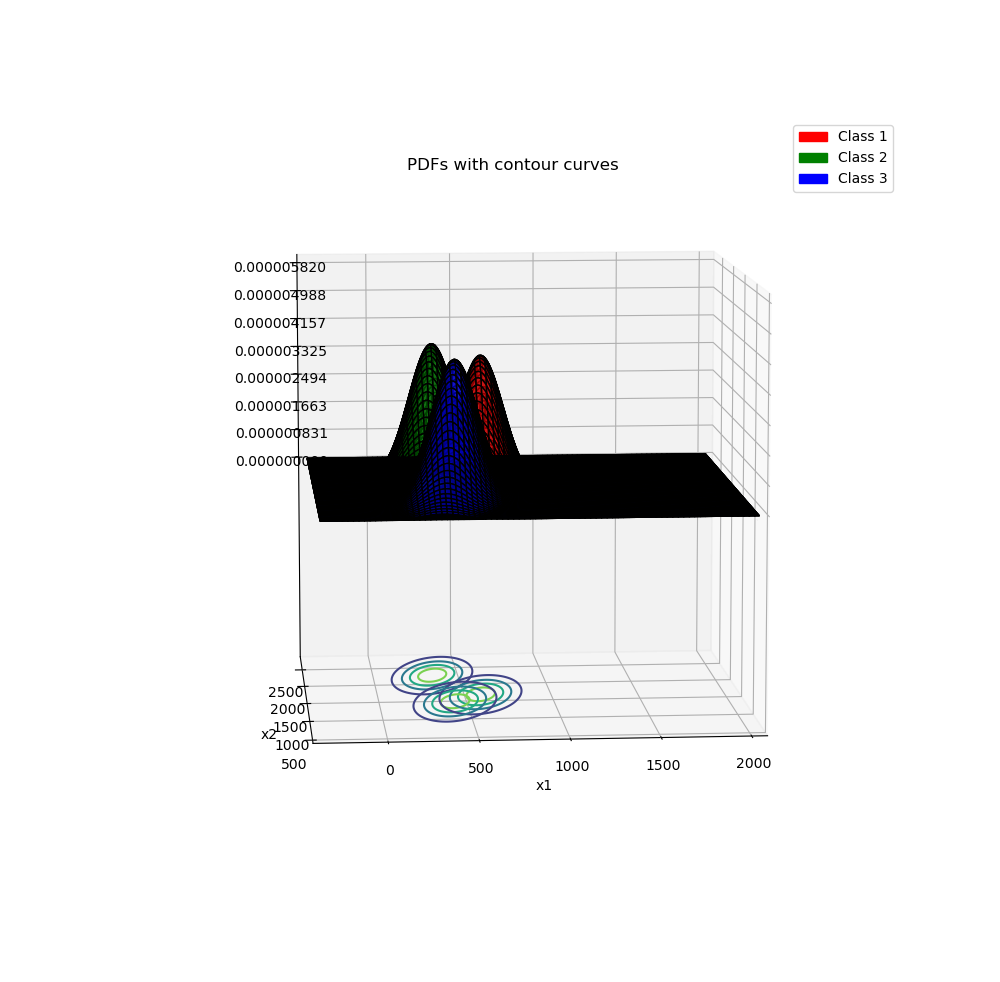
\includegraphics[width=5.5cm]{classifier/PDFs/REAL/case1.png}
  & 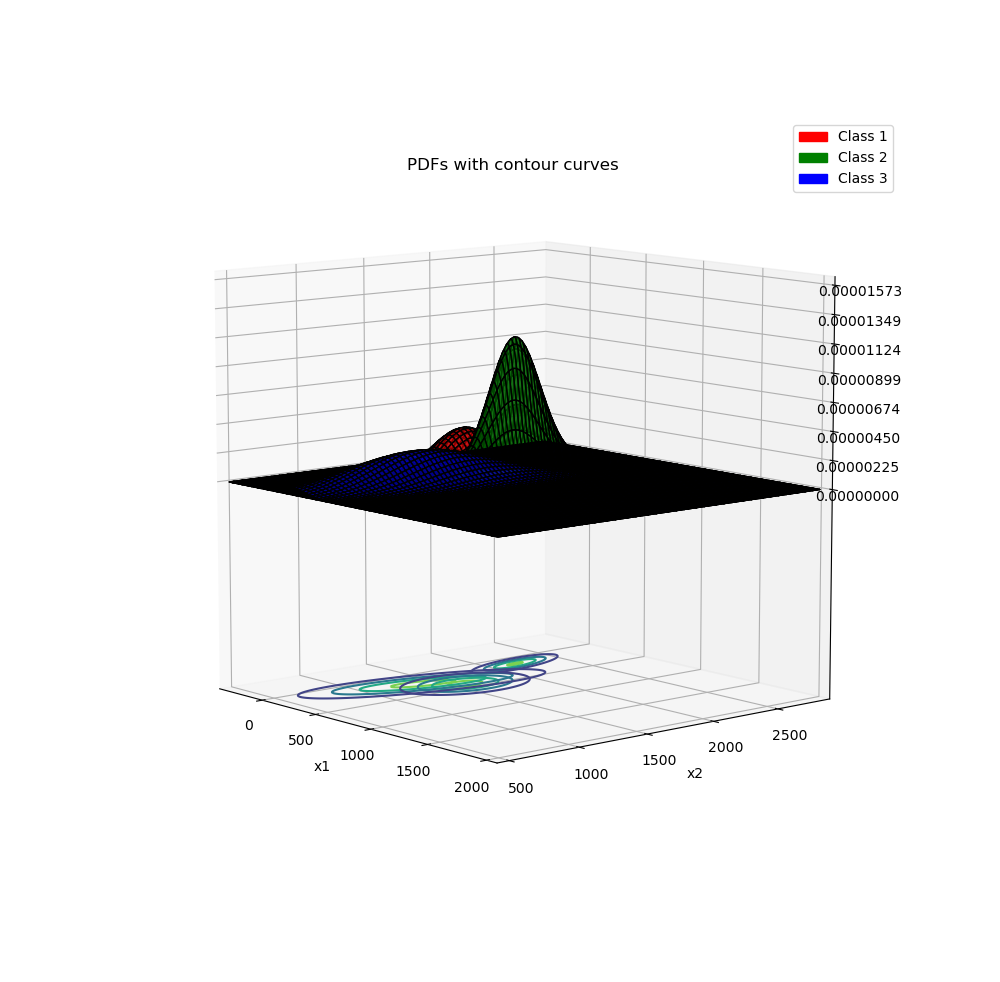
\includegraphics[width=5.5cm]{classifier/PDFs/REAL/case2.png}\\
  NLSC3 & NLSC5 & REC1 & REC2 \\
  \end{tabular}
  \captionof{figure}{Probability Density Function Plots}
\end{center}
 From figure 13, we can see that a) for NLSC3 and REC1, all 3 class pdfs share the same shape (they are just shifted forms of each other), b) from NLSC5 and REC2, we can see that a large covariance determinant leads to a flatter PDF.
 
\section*{Eigenvector and Contour Plots:-}

\begin{center}
  \setlength\tabcolsep{-4pt}
  \begin{tabular}{cccc}
  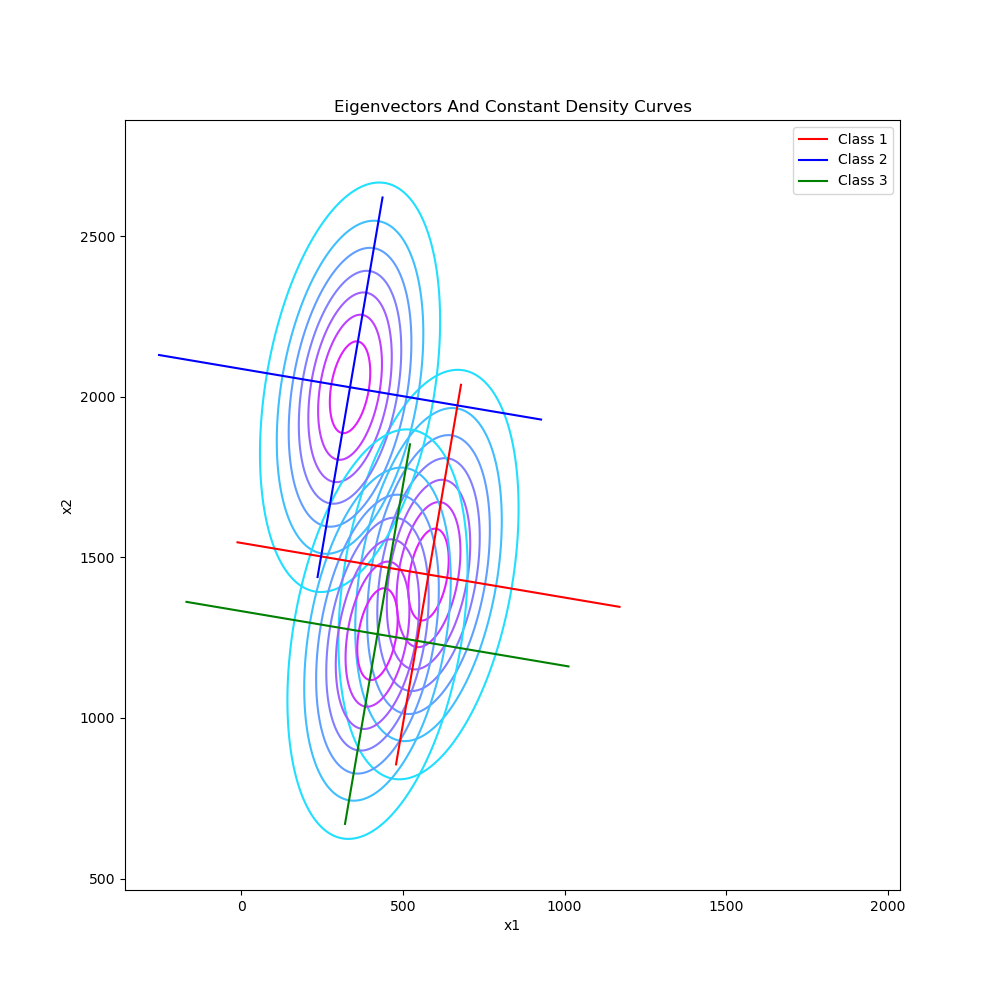
\includegraphics[width=4.5cm]{classifier/REAL_plots/EigenvectorContour_Case1.png}
  & 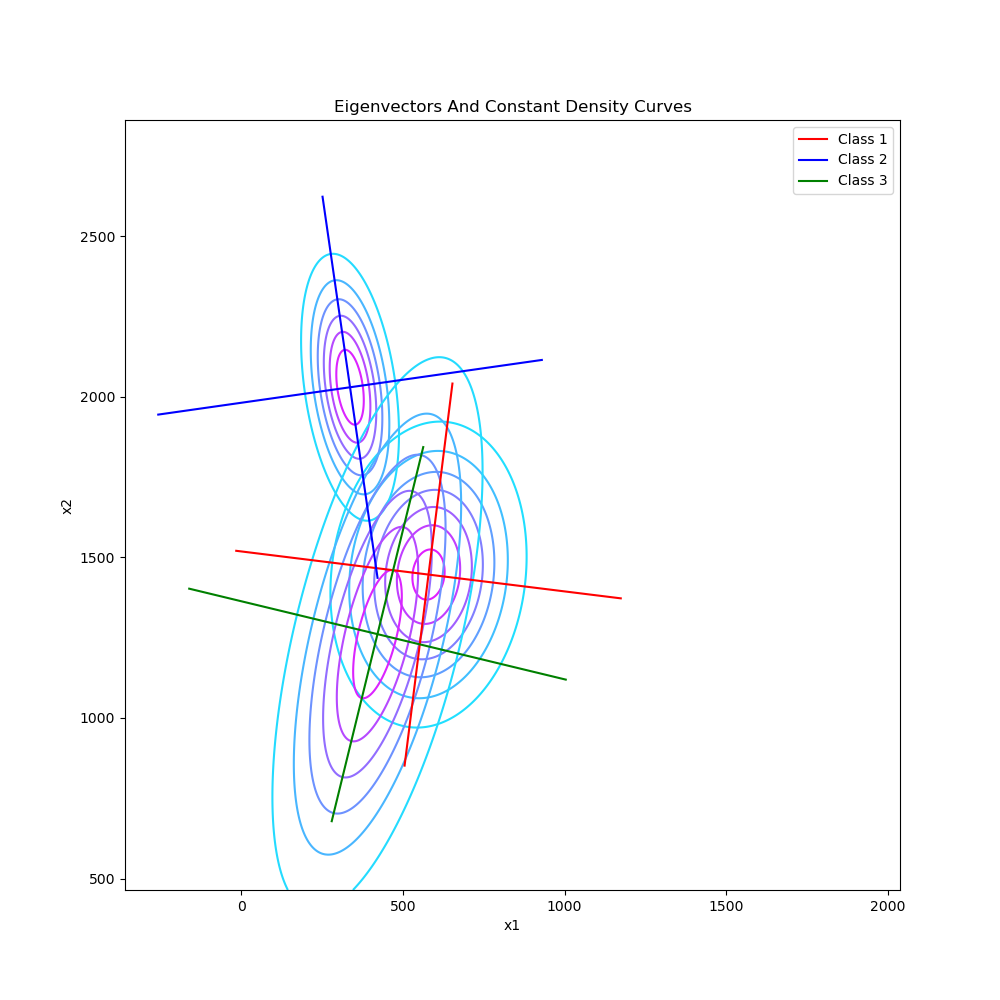
\includegraphics[width=4.5cm]{classifier/REAL_plots/EigenvectorContour_Case2.png}
  & 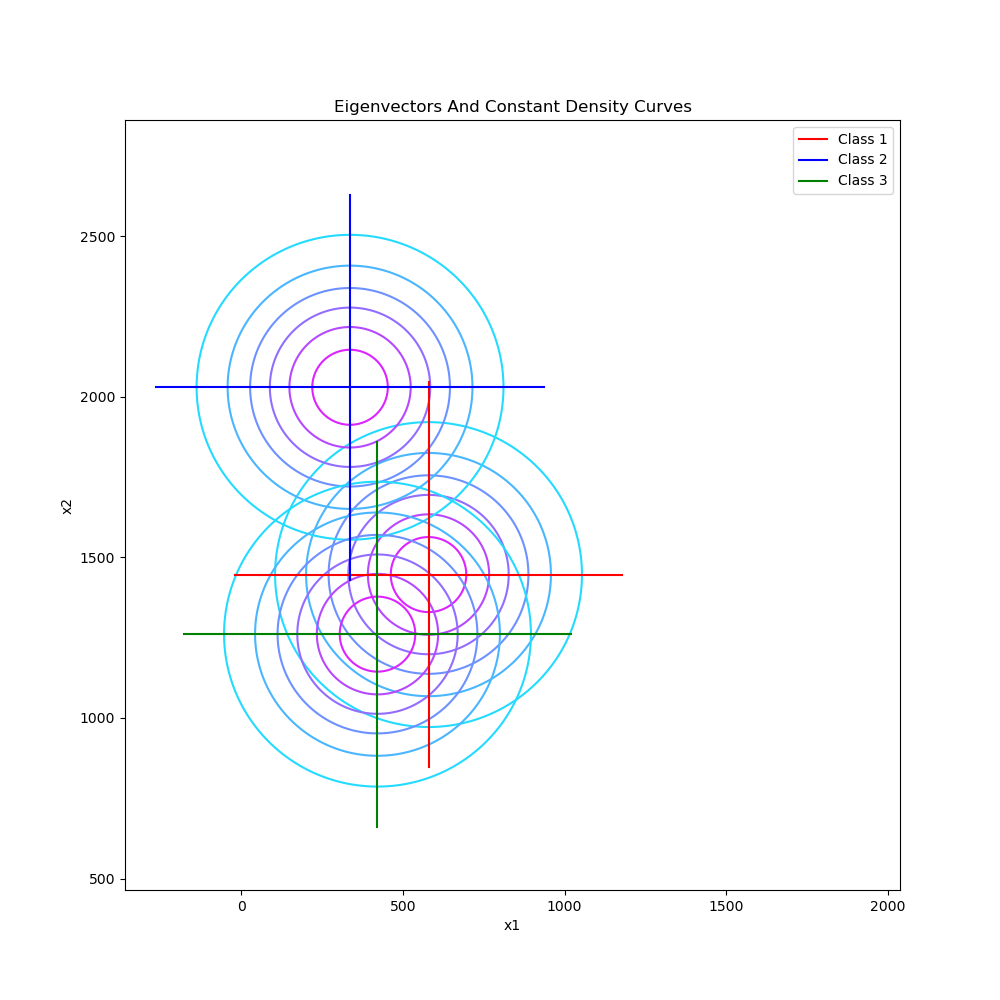
\includegraphics[width=4.5cm]{classifier/REAL_plots/EigenvectorContour_Case3.png}
  & 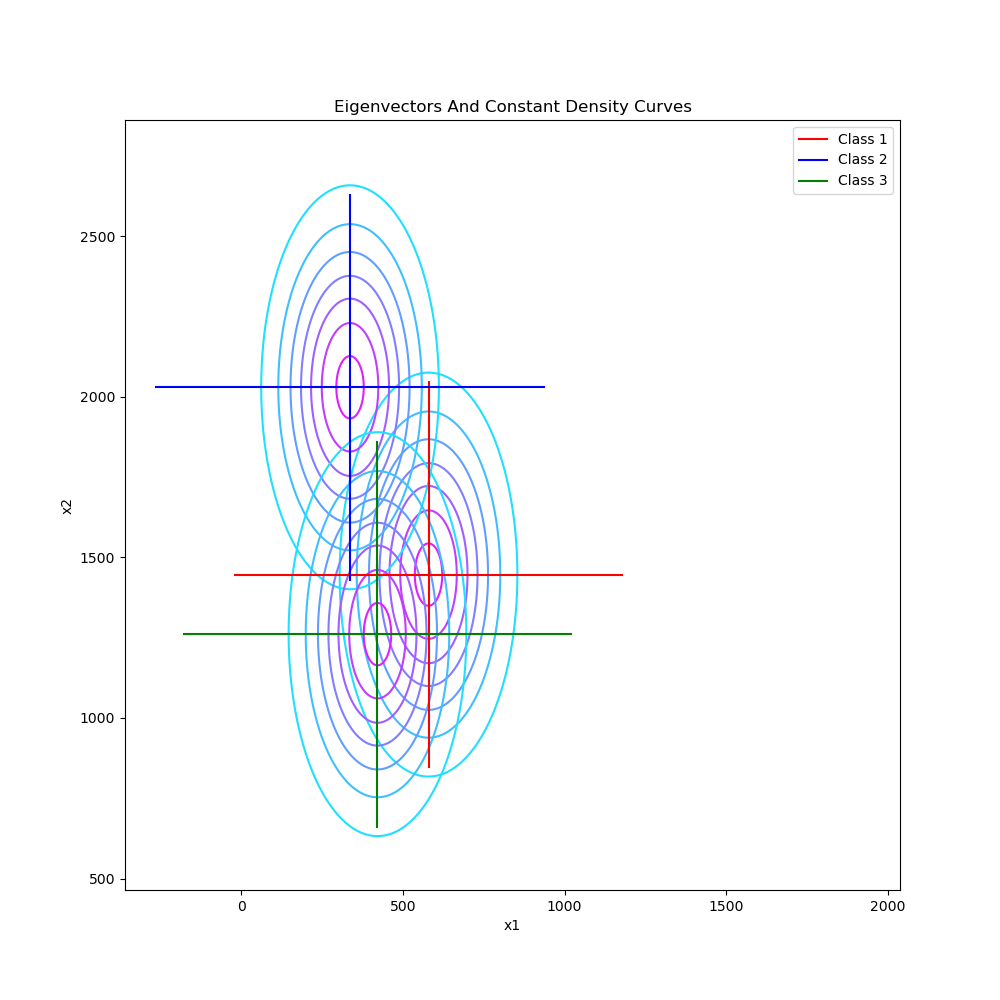
\includegraphics[width=4.5cm]{classifier/REAL_plots/EigenvectorContour_Case4.png} \\
  REC1 & REC2 & REC3 & REC4\\
  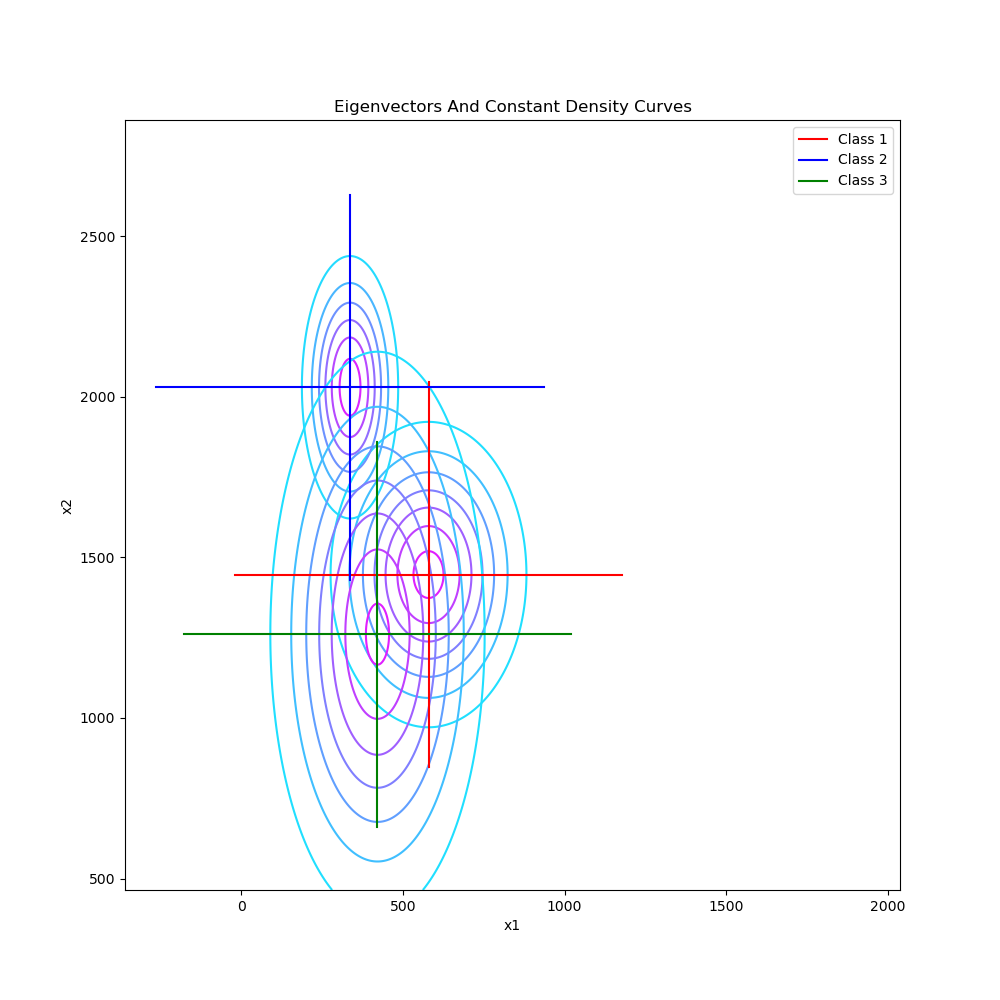
\includegraphics[width=4.5cm]{classifier/REAL_plots/EigenvectorContour_Case5.png}
  & 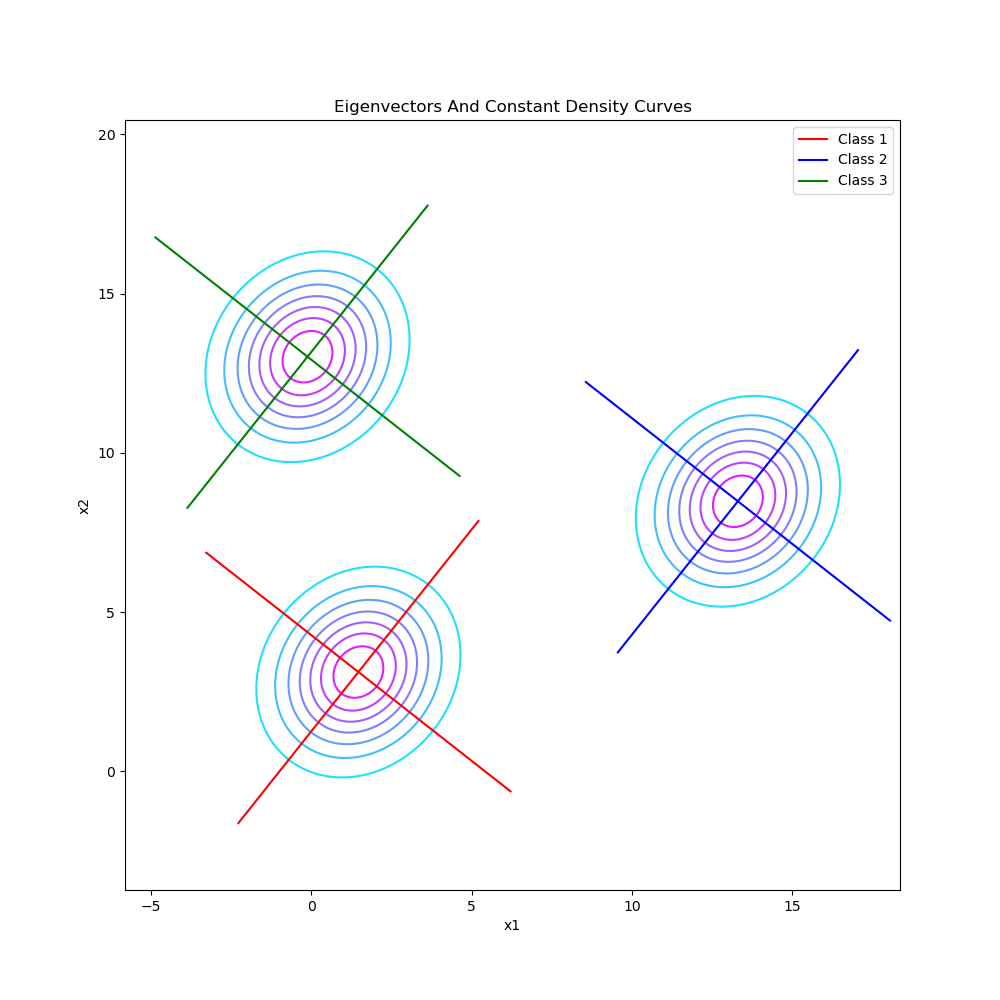
\includegraphics[width=4.5cm]{classifier/LS_plots/EigenvectorContour_Case1.png}
  & 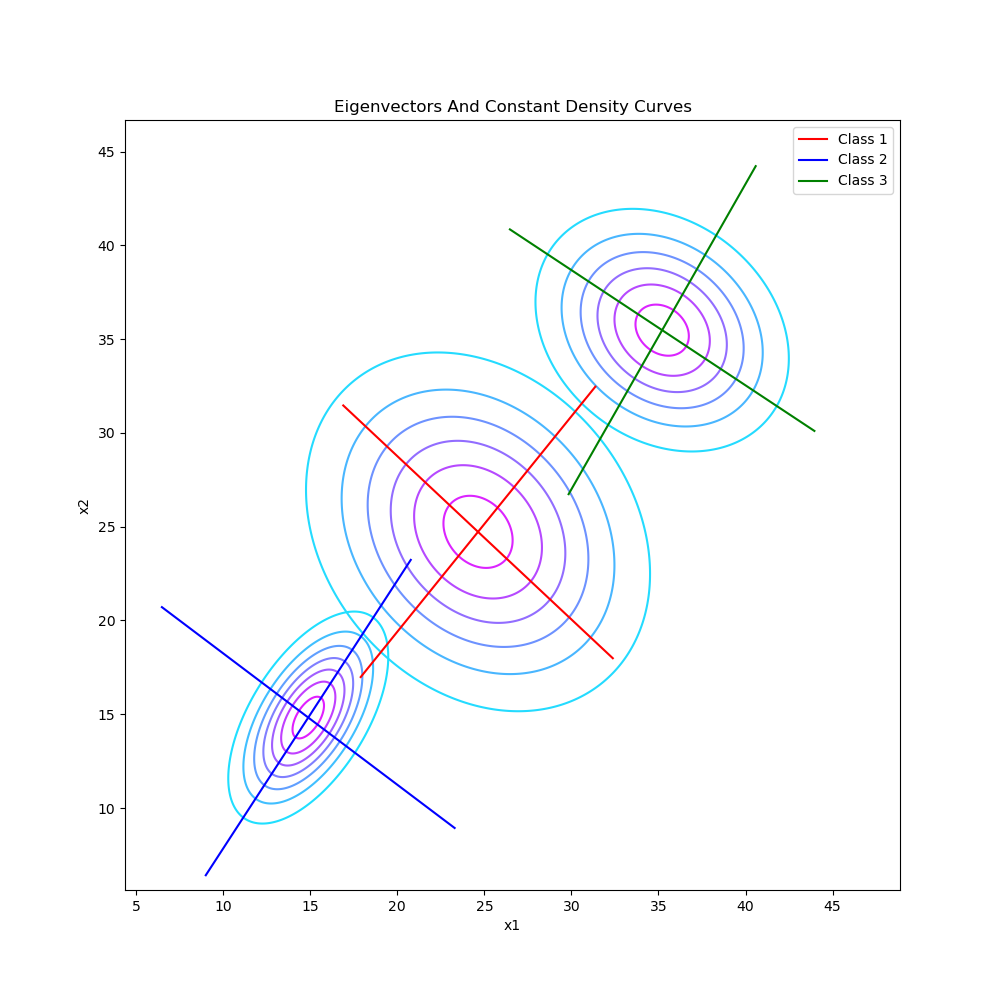
\includegraphics[width=4.5cm]{classifier/NLS_plots/EigenvectorContour_Case2.png} \\
  REC5 & LSC1 & NLSC2\\
  \end{tabular}
  \captionof{figure}{Eigenvector and Contour Curves Plots}
\end{center}
From figure 14, we note the following. For cases 1, 3, 4, where all classes share a covariance matrix, the contour ellipses of each class are the same (just shifted) and the eigenvectors of the covariance matrix are parallel. In cases 3, 4, 5, where we have a diagonal covariance matrix, the eigenvectors of every class is parallel to the co-ordinate axes. Also, a well-spread (large covariance determinant) indicates contours are more separated and enclose a larger area.

\section*{Decision Boundary Diagrams:-}

\begin{center}
  \setlength\tabcolsep{-4pt}
  \begin{tabular}{cccc}
  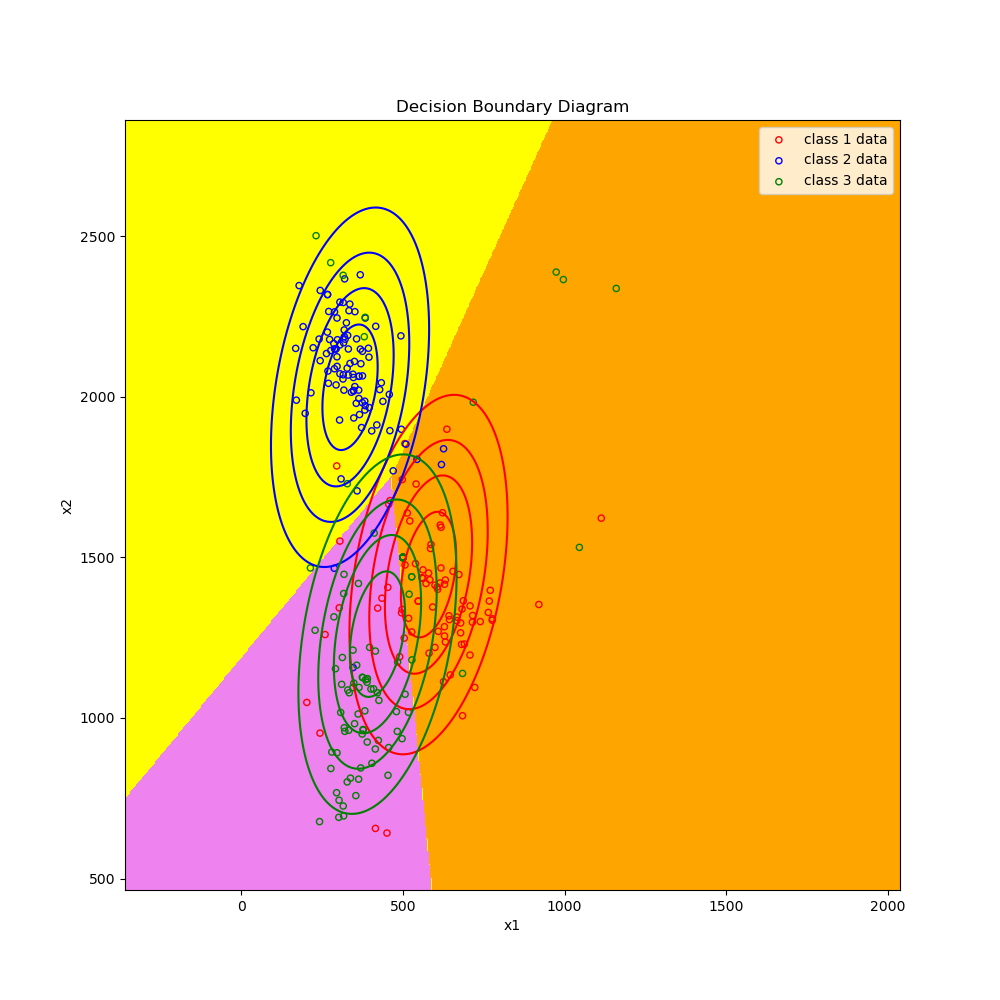
\includegraphics[width=4.5cm]{classifier/REAL_plots/DecisionBoundary_Case1.png}
  & 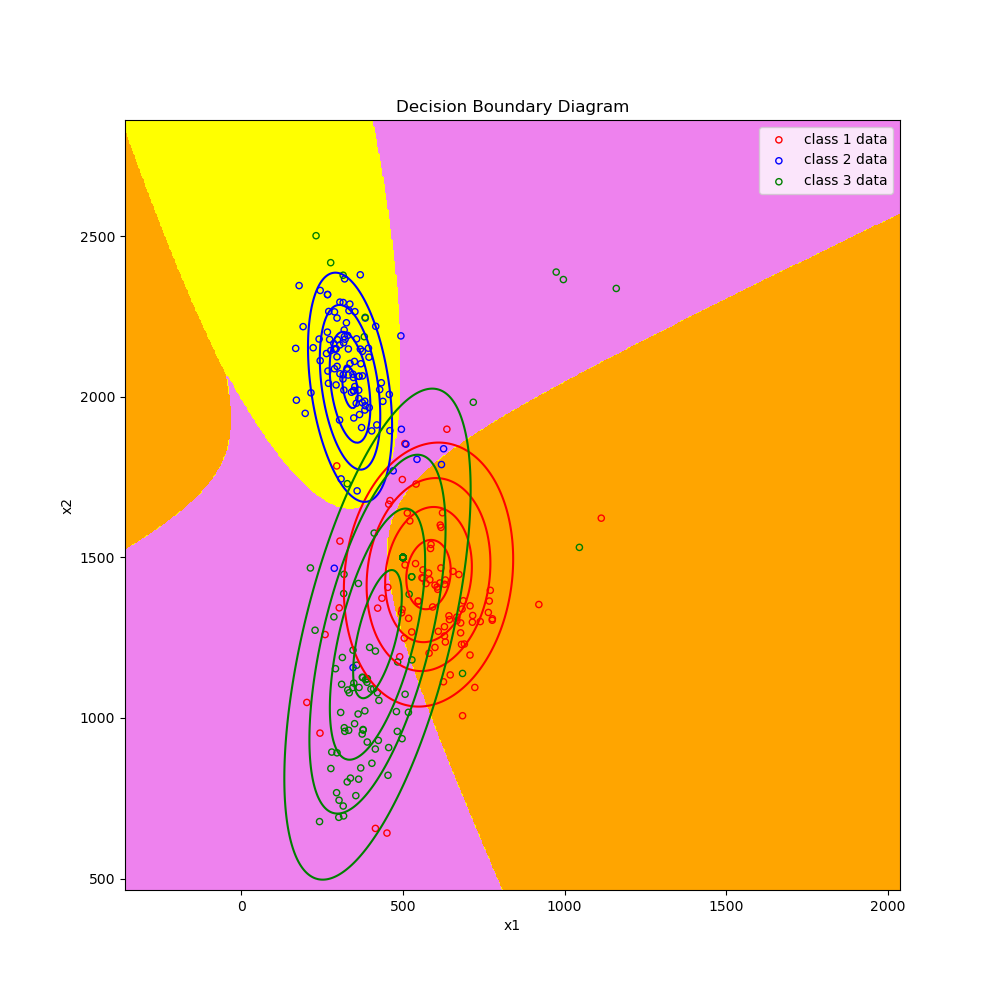
\includegraphics[width=4.5cm]{classifier/REAL_plots/DecisionBoundary_Case2.png}
  & 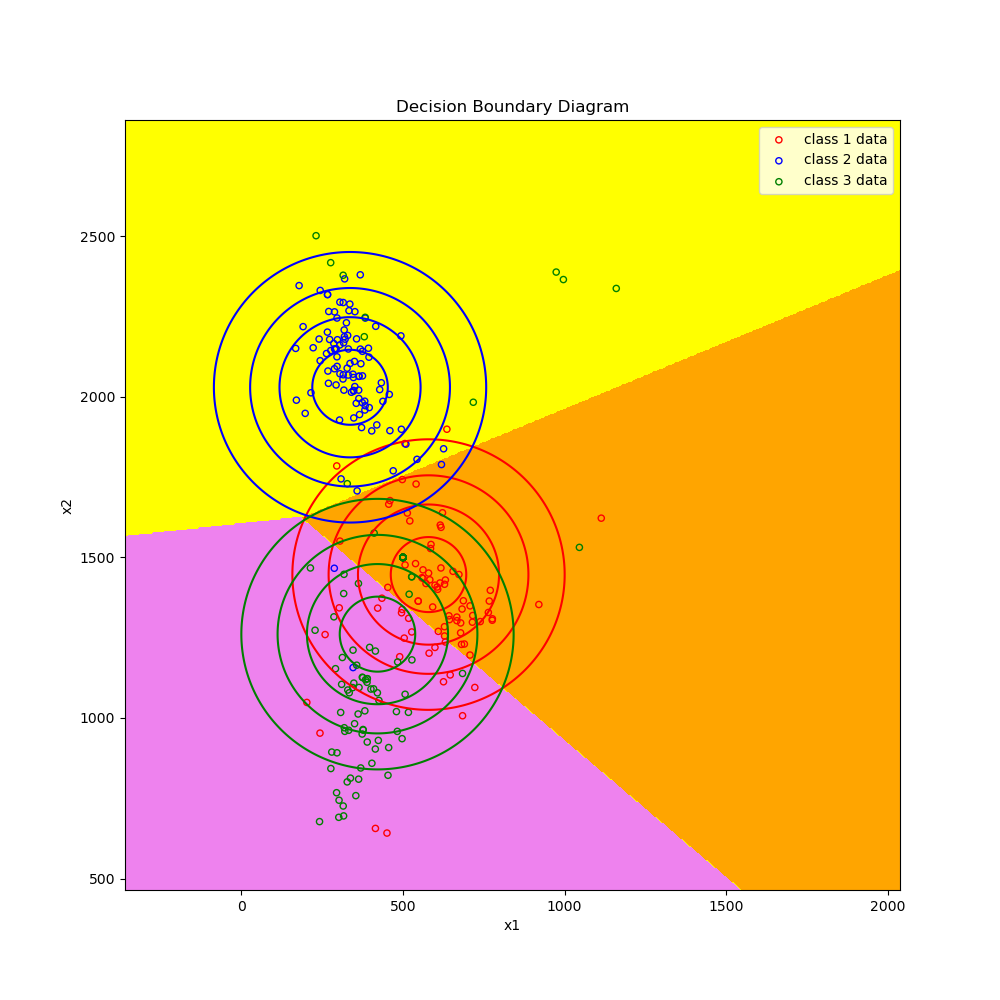
\includegraphics[width=4.5cm]{classifier/REAL_plots/DecisionBoundary_Case3.png}
  & 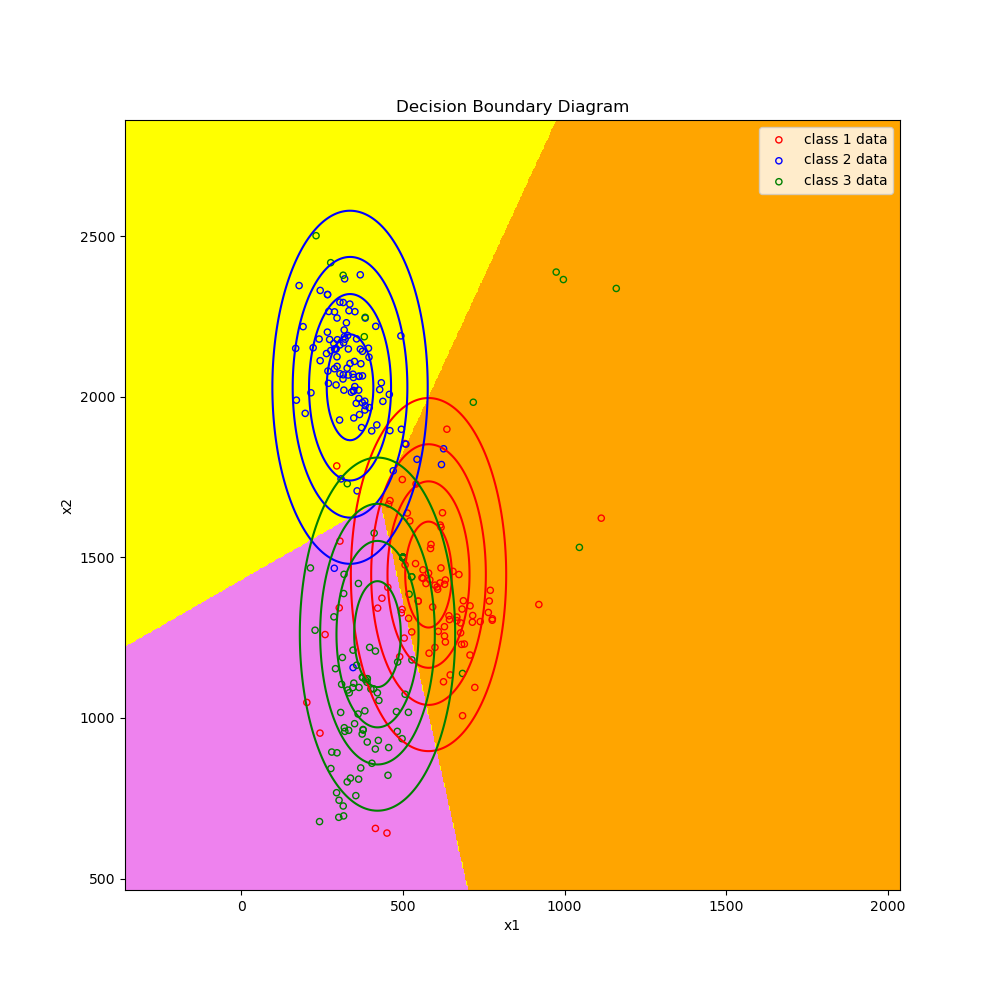
\includegraphics[width=4.5cm]{classifier/REAL_plots/DecisionBoundary_Case4.png} \\
  REC1 & REC2 & REC3 & REC4\\
  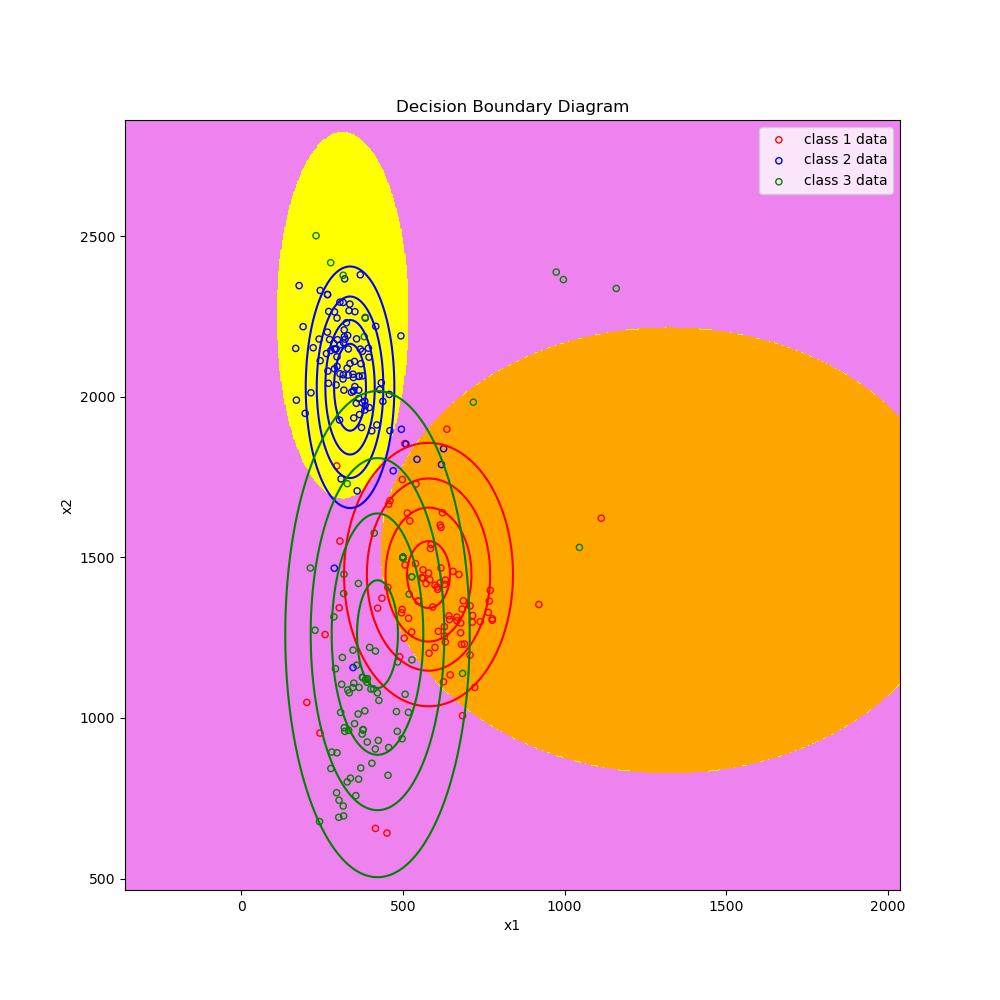
\includegraphics[width=4.5cm]{classifier/REAL_plots/DecisionBoundary_Case5.png}
  & 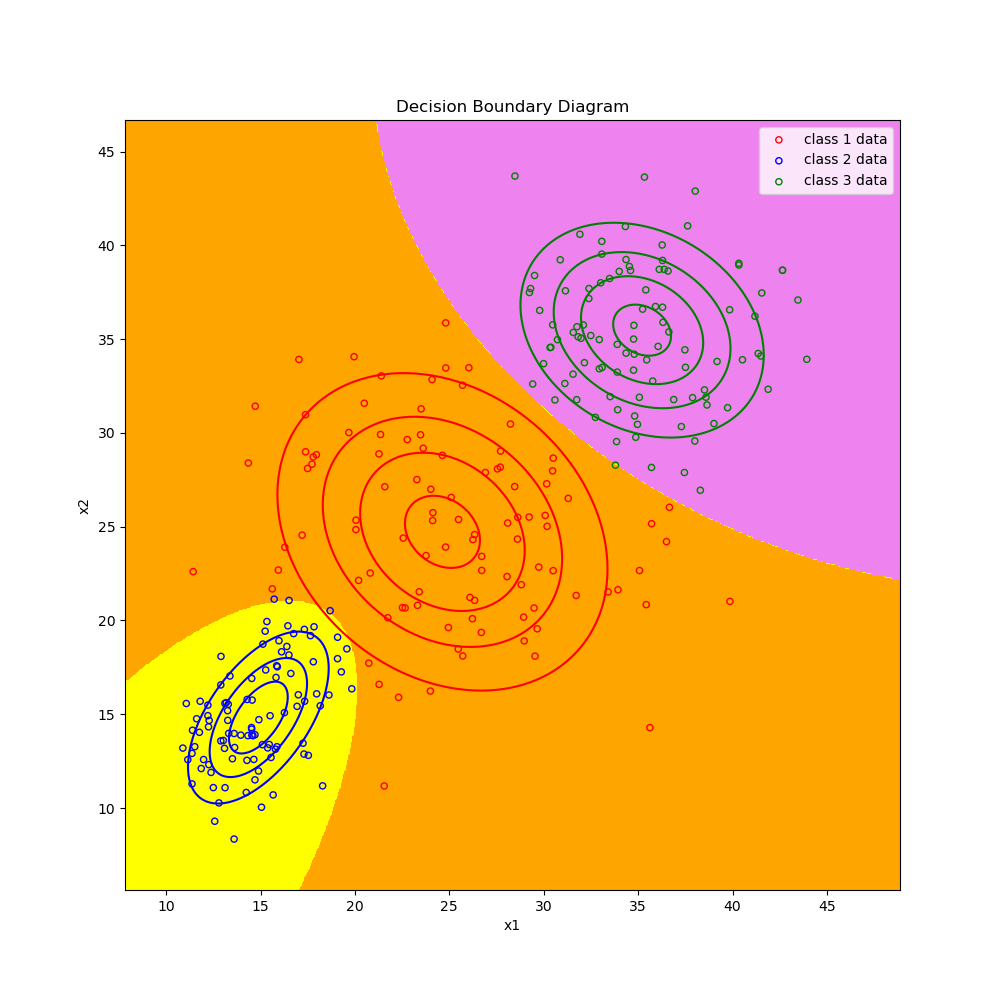
\includegraphics[width=4.5cm]{classifier/NLS_plots/DecisionBoundary_Case2.png}
  & 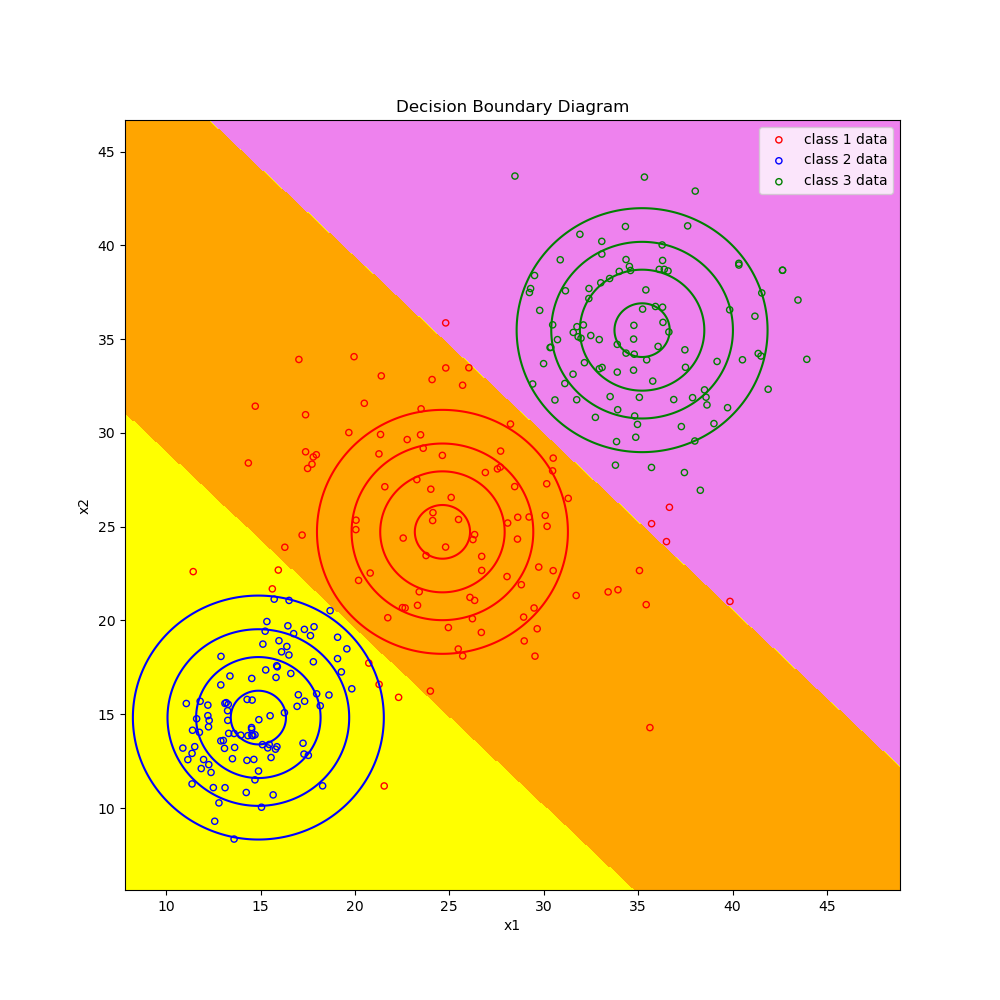
\includegraphics[width=4.5cm]{classifier/NLS_plots/DecisionBoundary_Case4.png}
  & 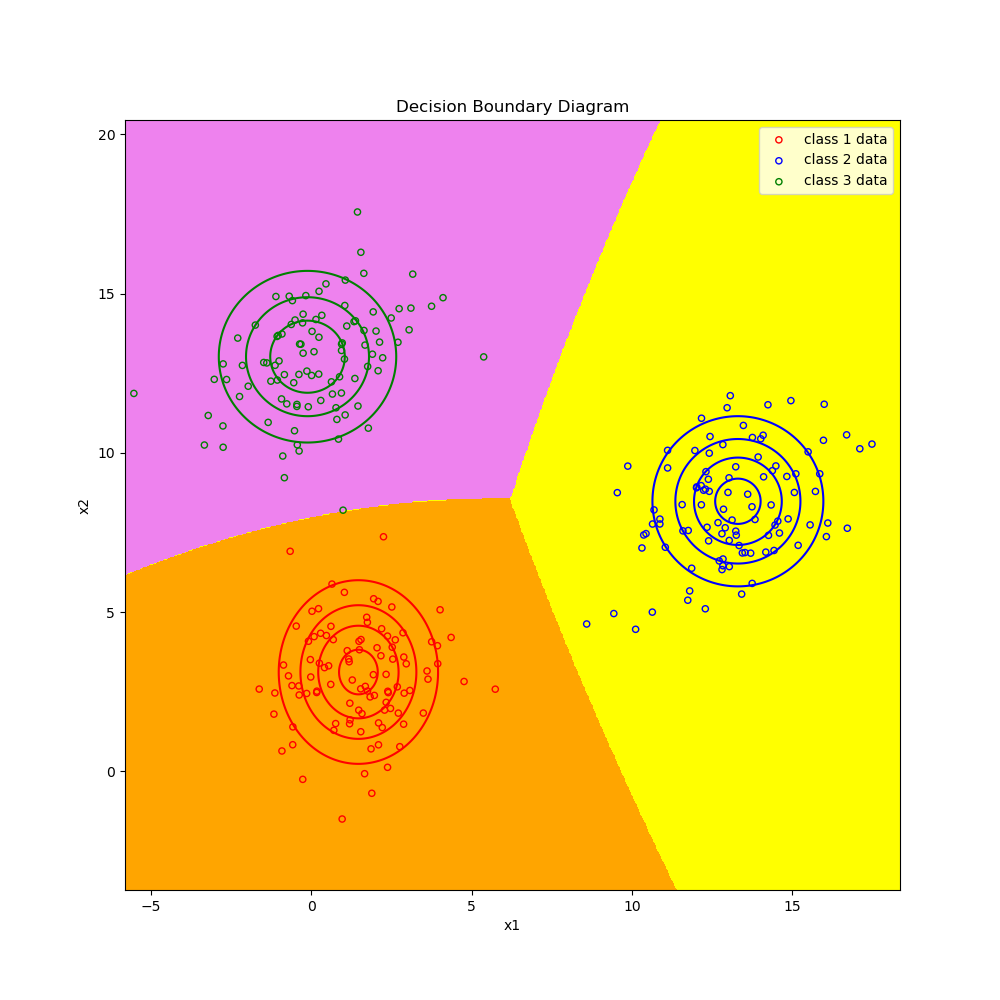
\includegraphics[width=4.5cm]{classifier/LS_plots/DecisionBoundary_Case5.png} \\
  REC5 & NLSC2 & NLSC4 & LSC5\\
  \end{tabular}
  \captionof{figure}{Decision Boundary Diagrams}
\end{center}
From figure 15, we can make several observations. We can see that quadratic decision boundaries will occur only when all classes are allowed to have different covariance matrices (cases 2 and 5). In cases 1, 3, 4, all decision boundaries are linear. In case 3, as the common covariance matrix is a multiple of the identity matrix, the contour curves of each class are concentric circles, the decision boundary between any 2 adjacent classes passes through the midpoint of their means and it is also perpendicular to the line joining the means. In cases 1, 4, where the classes just have a common covariance matrix, the decision boundary of 2 adjacent classes only passes through the midpoint. Classification using this diagram is also trivial - any development data point will belong to the class in whose shaded-region it lies.

\section*{Confusion Matrices:-}
\begin{center}
  \setlength\tabcolsep{0pt}
  \begin{tabular}{ccc}
  \includegraphics[width=4.5cm]{classifier/LS_plots/ConfusionMatrix_Case5.png}
  & \includegraphics[width=4.5cm]{classifier/NLS_plots/ConfusionMatrix_Case2.png}
  & \includegraphics[width=4.5cm]{classifier/REAL_plots/ConfusionMatrix_Case5.png} \\
  LSC5 & NLSC2 & REC5 \\
  \end{tabular}
  \captionof{figure}{Confusion Matrices}
\end{center}
For LS data, the confusion matrices were all the same as LSC5. No matter which technique we use, all classifiers get a $100\%$ accuracy. For NLS and RE data, the misclassification rates are quite high (especially for RE) which is indicated by the off-diagonal entries being non-zero (quite large numbers for RE).

\section*{ROC-DET curves:-}
\begin{center}
  \setlength\tabcolsep{0pt}
  \begin{tabular}{cc}
  \includegraphics[height=5cm,width=10cm]{classifier/LS_plots/ROCDETPlot.png}
  & \includegraphics[height=5cm,width=10cm]{classifier/NLS_plots/ROCDETPlot.png} \\
  LSROCDET & NLSROCDET \\
  \end{tabular} \\
  \begin{tabular}{c}
  \includegraphics[height=9cm,width=18cm]{classifier/REAL_plots/ROCDETPlot.png} \\
  REROCDET \\
  \end{tabular}
  \captionof{figure}{ROC-DET Plots}
\end{center}

For LS data, all the 5 cases have a good ROC. Excellent operating points, which are close to $(0,1)$, can be picked for each of the 5 cases. This is because of the fact that the data is linearly separable.

For NLS data, the ROC curves for all cases are now less than ideal. From the ROC curve, it can be seen that case 2 (the most relaxed assumption case) is a better choice than the other cases. A good operating point, determined by looking at the DET curve (as this provides a better look at the error rates), can be taken around $(4\%, 4\%)$.

For RE data, the ROC curves of all cases are far from ideal. No case performs comfortably better than the others. This is primarily because of the fact that this is actual data extracted from real sources. This data exhibits the general trend of the ROC curve in real-life classification scenarios, i.e, at large thresholds - both TPR and FPR are close to 0 (as no data is classified as Positive), with a decrease in threshold - both TPR and FPR increase and at small thresholds - both TPR and FPR are close to 1. 
\end{document}
